\chapter{Arhitektura i dizajn sustava}
		
	Da bi dugoročno uštedjeli vrijeme, uložili smo dio vremena na konfiguriranje CI (engl. continuous integration) i CD (engl. continuous delivery) procesa. Za isporuku aplikacije odabrali smo Heroku.
	
	Heroku je jedna od najpoznatijih platformi za isporučivanje aplikacija koja se ističe svojom jednostavnošću. Za razliku od AWS-ovih servisa, koje smo također razmatrali, Heroku se sam brine oko instanci i arhitekture sustava na kojem se izvodi naša aplikacija. Zbog ograničenih resursa odlučili smo isporučiti aplikaciju na besplatnu instancu Heroku-a.
	
	Besplatna instanca Heroku-a ima određena ograničenja, a najupečatljivije od njih je način na koji se pokreće projekt.
	Heroku sam prepoznaje kojeg je tipa projekt pa da pokrenemo frontend i backend trebamo dvije instance.
	CD je integriran putem GitLab-ovih pipelinesa za koje je bilo potrebno napisati .gitlab-ci.yml datoteku u kojoj smo konfigurirali GitLab-ov pipeline. GitLab-ov pipeline konfiguriran je tako da se na svaki commit u dev grani izgradi aplikacija, pokrenu i uspješno završe testovi te krene isporuka aplikacije na Heroku.
	
	Da bi osigurali maksimalno vrijeme dostupnosti naše platforme, .yml datoteka također je konfigurirana tako da prilikom commita u master isporuči aplikaciju na druge dvije instance.
	Ukupno imamo četiri pokrenute instance Heroku-a, od koje su dvije backend, a dvije frontend. Backend i frontend imaju svaki svoju razvojnu i produkcijsku instancu. Poveznice na instance:
	\begin{itemize}
		\item \url{http://giger-fer.herokuapp.com/}
		\item \url{https://giger-fer-dev.herokuapp.com/}
		\item \url{https://giger-backend-dev.herokuapp.com/}
		\item \url{http://giger-backend.herokuapp.com/}
	\end{itemize}
	
	
	U skladu s time, Spring Boot aplikacija ima dvije .properties datoteke. Jedna od njih je namijenjena lokalnom izvođenju aplikacije te sadrži postavke lokalne PostgreSQL baze, dok je druga konfigurirana tako da postavke čita iz varijabli okruženja. Varijable okruženja postavljene su na Heroku tako da čak niti pristupom u git repozitorij vanjski korisnik ne može doći do akreditacije (credentials) kojima bi mogao pristupiti bazi.
	
	Prednost ostvarena automatiziranjem procesa isporuke jest povećanje vjerojatnosti uspješnosti iste te povećanje udjela dostupnosti aplikacije zbog dva para instanci servera.
	
	Uvidjevši prednosti korištenja CD-a, primijenili smo to znanje i na prevođenje dokumentacije. 
	Unutar repozitorija, osim pipeline-a za isporuku aplikacije, postoji pipeline za automatsko prevođenje dokumentacije čiji je rezultat .pdf dokument.\\
	Potencijalni prostor za napredak bio bi korištenje Docker tehnologije tako da prilikom pokretanja aplikacije korisnik ne mora imati instaliranu PostgreSQL bazu već ju pokrene u Docker kontejneru.
	
	Od mogućih arhitektura sustava, za svoj projekt smo odabrali objektno usmjerenu arhitekturu. Tu arhitekturu smo odabrali zato što se koristi u industriji te je de facto standard razvoja složenih programskih rješenja. Osim toga, ona je fleksibilna, omogućuje recikliranje koda te logički razdjeljuje sustav na više cjelina, što je bitno s obzirom da više ljudi radi na implementaciji aplikacije. Zahvaljujući modularnosti programskog rješenja, greške su lako ispravljive, a nove mogućnosti dodaju se bez poteškoća.

	Odlučili smo se za web aplikaciju, koja je prilagođena mobilnim uređajima, obzirom da glazbenici, a time i bendovi nemaju uvijek pristup računalu, a ne želimo da je korisnik ograničen samo na mobilne uređaje.\\

	Arhitekturu sustava možemo podijeliti na četiri podsustava:
		\begin{itemize}
			\item Web preglednik
			\item Web poslužitelj
    			\item Web aplikacija
			\item Baza podataka
		\end{itemize}

	
	
	Korisnik (javnost, glazbenik, bend, administrator) pristupa web aplikaciji uz pomoć svog web preglednika, s time da se u sredini nalazi web poslužitelj. Na njemu se nalazi aplikacija koju on pokreće, te uz pomoć protokola komunicira s korisnicima.

	Klijentski (frontend) dio aplikacije omogućuje da korisnik korištenjem sučelja može pristupiti serveru (backend) aplikacije. Ovisno o tome što korisnik hoće, taj server ima mogućnost spajanja na bazu podataka kako bi korisniku prikazao informacije.

	Backend je napisan u Javi 11, a kao razvojni okvir koristimo Java Spring Boot 2.2.0. Dodani su projekti Spring Data JPA kako bi backend mogao lako komunicirati s bazom, Spring Web MVC za rukovanje zahtjevima te Spring Security kako bi zaštitili aplikaciju od vanjskih napada. Za pregledniji kod koristimo Lombok.

	\begin{figure}[H]
		\begin{center}
			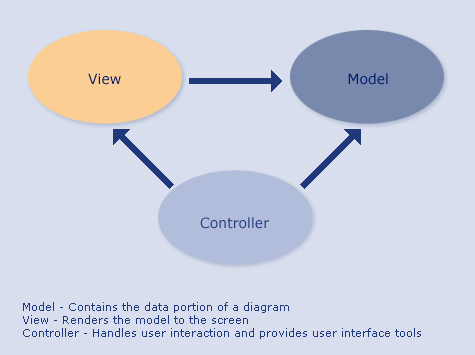
\includegraphics[width=10cm]{slike/mvc.PNG}
		\end{center}
		\caption{Pojednostavljeni prikaz MVC-a}
		\label{fig:mvc}
	\end{figure}

	Za frontend koristimo React. On je moderan i jednostavan framework koji koristi HTML, CSS, JSX i JavaScript uz pomoć kojeg smo napravili sučelje za našu aplikaciju. Uz pomoć React-a možemo lagano komunicirati s backendom koristeći REST.\\




		\section{Baza podataka}
		Za potrebe razvoja \textit{Gigera} koristit će se objektno relacijsko mapiranje. To je metoda koja se koristi u objektno-orijentiranim jezicima te se na taj način stvara virtualna objektna baza podataka. Za implementaciju baze podataka odabrali smo PostgreSQL, zbog generalno pozitivnog iskustva u korištenju te implementacije baze podataka u dosadašnjem fakultetskom obrazovanju. Bitno je naglasiti da na osobnim računalima u svrhu razvijanja aplikacije koristimo istu implementaciju baze kao i na web poslužitelju kako bi minimizirali neočekivano ponašanje.
		
		Baza podataka sastoji se od sljedećih tablica:
		
		\begin{packed_item}
		\item Message
		\item Conversation\_messages
		\item Conversation
		\item Conversation\_participants
		\item System\_person
		\item Person
		\item System\_person\_roles
		\item Organizer
		\item Band 
		\item Band\_occasions
		\item Occasion
		\item Musician\_occasions
		\item Band\_invited\_back\_up\_members
		\item Band\_invited 
		\item Band\_back\_up\_members
		\item Band\_members
		\item Band\_acceptable\_gig\_types
		\item Band\_invitation\_gigs
		\item Band\_gigs
		\item Band\_posts	
		\item Gig
		\item Gig\_reviews
		\item Review
		\item Post
		\item Post\_comments
		\item Comment
		\item Musician
		\item Musician\_instruments
		\item Instrument
		\item Musician\_past\_gigs
		
		
	\end{packed_item}
	
	
	\subsection{Opis tablica}
	
	\textbf{Message}
	Ovaj entitet sadrži informacije o poruci. Sadrži atribute: id poruke, sadržaj poruke, vrijeme kada je poruka poslana, id pošiljatelja i id razgovora. Ovaj entitet je u \textit{Many-to-One} vezi s entitetima: Conversation, Person, Band. Ako je bend poslao poruku, tada je fk\_sender null, a ako ju je poslao korisnik tada je fk\_sender\_band null.
	\begin{longtabu} to \textwidth {|X[6, l+3]|X[6, l]|X[20, l]|}
		
		\hline \multicolumn{3}{|c|}{\textbf{Message}}	 \\[3pt] \hline
		\endfirsthead
		
		\hline
		\endlastfoot
		
		\textbf{id} & BIGINT	&  	jedinstveni identifikator poruke 	\\ \hline
		content	& VARCHAR & sadržaj poruke	\\ \hline
		sent\_time & TIMESTAMP & vrijeme kada je poruka poslana \\ \hline
		\textit{sender\_id} & BIGINT & jedinstveni identifikator pošiljatelja \\ \hline
		\textit{sender\_band\_id} & BIGINT & jedinstveni identifikator benda pošiljatelja \\ \hline

		
	\end{longtabu}

		\textbf{Conversation\_messages}
	
	\begin{longtabu} to \textwidth {|X[6, l+3]|X[6, l]|X[20, l]|}
		
		\hline \multicolumn{3}{|c|}{\textbf{Conversation\_messages}}	 \\[3pt] \hline
		\endfirsthead
		
		\hline
		\endlastfoot
		
		\textbf{conversation\_id}	& BIGINT &  jedinstveni identifikator razgovora	\\ \hline
		\textbf{messages\_id} & BIGINT	&  	jedinstveni identifikator poruke razgovora \\ \hline
		
		
	\end{longtabu}
	
	\textbf{Conversation}
	Ovaj entitet sadrži informacije o razgovoru. Sadrži atribute: id razgovora i ime razgovora. Ovaj entitet je u \textit{One-to-Many} vezi s entitetima: Message i
	\emph{Many-to-One} vezi s entitetima: Band i Person.
	\begin{longtabu} to \textwidth {|X[6, l+3]|X[6, l]|X[20, l]|}
		
		\hline \multicolumn{3}{|c|}{\textbf{Conversation}}	 \\[3pt] \hline
		\endfirsthead
		
		\hline
		\endlastfoot
		
		\textbf{id} & BIGINT	&  	jedinstveni identifikator razgovora 	\\ \hline
		picture\_url & VARCHAR & url slike razgovora \\ \hline
		title	& VARCHAR &  naziv razgovora	\\ \hline
		\textit{band\_id} & BIGINT & jedinstveni identifikator benda \\ \hline
		
		
		
	\end{longtabu}
	
	\textbf{Conversation\_participants}
	Ova vezna tablica sadrži informacije o sudjelovanju korisniku u razgovoru. Sadrži atribute: id korisnika i id razgovora.
	\begin{longtabu} to \textwidth {|X[6, l+3]|X[6, l]|X[20, l]|}
		
		\hline \multicolumn{3}{|c|}{\textbf{Conversation\_participants}}	 \\[3pt] \hline
		\endfirsthead
		
		\hline
		\endlastfoot
		
		\textbf{conversation\_id}	& BIGINT &  jedinstveni identifikator razgovora	\\ \hline
		\textbf{participants\_id} & BIGINT	&  	jedinstveni identifikator korisnika koji sudjeluje u razgovoru \\ \hline
		
		
	\end{longtabu}
	
	\textbf {System\_person}
	Ovaj entitet sadrži podatke korisnika potrebne sustavu za sistemsku logiku.  Sadrži atribute: id korisnika, email, locked i verified zastavice te šifriranu lozinku. Ovaj entitet je u \emph{One-to-Many} vezi s entitetom: Roles i \emph{One-to-One} vezi s entitetima: Person, Musician i Organizer.
	\begin{longtabu} to \textwidth {|X[6, l+3]|X[6, l]|X[20, l]|}
		
		\hline \multicolumn{3}{|c|}{\textbf{System\_person}}	 \\[3pt] \hline
		\endfirsthead
		
		\hline
		\endlastfoot
		
		\textbf{id} & BIGINT	&  	jedinstveni identifikator sustavskih podataka o korisniku	\\ \hline
		email & VARCHAR & email adresa osobe \\ \hline
		locked & BOOLEAN & korisnik ima zabranu korištenja aplikacije ili ne \\ \hline
		password\_hash & VARCHAR & hash lozinke osobe \\ \hline
		verified & BOOLEAN & email adresa potvrđena ili ne \\ \hline
		
	\end{longtabu}
	
		\textbf{Person}
	Ovaj entitet sadrži podatke korisnika potrebne za poslovne svrhe.  Sadrži atribute: telefonski broj, url slike korisnika, korisničko ime kojim se predstavlja javnosti. Ovaj entitet je u \emph{One-to-Many} vezi s entitetima: Conversation, Message i
	\emph{One-to-One} vezi s entitetima: Musician, System\_person i Organizer.
	\begin{longtabu} to \textwidth {|X[6, l+3]|X[6, l]|X[20, l]|}
		
		\hline \multicolumn{3}{|c|}{\textbf{Person}}	 \\[3pt] \hline
		\endfirsthead
		
		\hline
		\endlastfoot
		
		\textbf{id} & BIGINT	&  	jedinstveni identifikator korisnika	\\ \hline
		phone\_number & VARCHAR & telefonski broj korisnika \\ \hline
		picture\_url & VARCHAR & url slike korisnika \\ \hline
		username & VARCHAR & korisničko ime korisnika
		
	\end{longtabu}
	
		\textbf{System\_person\_roles}
	Ovo je vezna tablica koja sadrži n-torke iz kojih možemo iščitati dodijeljene uloge pojedinim korisnicima. Sadrži atribute: system\_person\_id i cijeli broj uloge koji predstavlja enumeraciju.
	\begin{longtabu} to \textwidth {|X[6, l+3]|X[6, l]|X[20, l]|}
		
		\hline \multicolumn{3}{|c|}{\textbf{System\_person\_roles}}	 \\[3pt] \hline
		\endfirsthead
		
		\hline
		\endlastfoot
		
		\textbf{system\_person\_id} & BIGINT	&  	jedinstveni identifikator sustavskih podataka o korisniku	\\ \hline
		\textbf{roles} & INT & uloga korisnika \\ \hline
		
		
	\end{longtabu}
	
	\textbf {Organizer}
	Ovaj entitet sadrži informacije o organizatoru. Sadrži atribute: id organizatora te ime organizatora. Ovaj entitet je u \emph{One-to-One} vezi s entitetima: Musician, System\_person i Organizer te u \emph{One-to-Many} vezi s entitetom Gig.
	\begin{longtabu} to \textwidth {|X[6, l+3]|X[6, l]|X[20, l]|}
		
		\hline \multicolumn{3}{|c|}{\textbf{Organizer}}	 \\[3pt] \hline
		\endfirsthead
		
		\hline
		\endlastfoot
		
		\textbf{id} & BIGINT	&  	jedinstveni identifikator organizatora 	\\ \hline
		manager\_name	& VARCHAR &  ime organizatora	\\ \hline
		
	\end{longtabu}

\textbf{Band}
Ovaj entitet sadrži podatke o kreiranom bendu.  Sadrži atribute: id, opis, datum formiranja, adresu sjedišta, dodatni opis adrese, par koordinata, maksimalnu udaljenost, naziv benda, url slike benda i id voditelja benda. Ovaj entitet je u \textit{Many-to-Many} vezi s Musician za potrebe liste članova, u \textit{Many-to-One} vezi s Musician za potrebu evidencije voditelja benda te \emph{One-to-Many} vezi s entitetima: Message, Conversation, Gig i Post.

	\begin{longtabu} to \textwidth {|X[6, l+3]|X[6, l]|X[20, l]|}
		
		\hline \multicolumn{3}{|c|}{\textbf{Band}}	 \\[3pt] \hline
		\endfirsthead
		
		\hline 
		\endlastfoot
		
		\textbf{id} & BIGINT	&  	jedinstveni identifikator benda 	\\ \hline
		bio & VARCHAR & opis benda \\ \hline
		formed\_date & DATE & datum osnutka benda \\ \hline
		address & VARCHAR & adresa benda \\ \hline
		extra\_description & VARCHAR & dodatak opis benda \\ \hline
		x & DOUBLE & x koordinata lokacije \\ \hline
		y & DOUBLE & y koordinata lokacije \\ \hline
		max\_distance & DOUBLE & najveća udaljenost koju bend želi prijeći zbog gaže \\ \hline
		name & VARCHAR & ime benda \\ \hline
		picture\_url & VARCHAR & url slike benda \\ \hline
		\textit{leader\_id}	& BIGINT &  jedinstveni identifikator voditelja benda	\\ \hline 	
		
	\end{longtabu}
	
				\textbf {Band\_occasions}
	Ovo je vezna tablica iz koje se može iščitati zauzetost benda. Sadrži atribute: identifikator benda i identifikator događaja.
	\begin{longtabu} to \textwidth {|X[6, l+3]|X[6, l]|X[20, l]|}
		
		\hline \multicolumn{3}{|c|}{\textbf{Band\_occasions}}	 \\[3pt] \hline
		\endfirsthead
		
		\hline
		\endlastfoot
		
		\textbf{band\_id} &  BIGINT	&  	jedinstveni identifikator benda koji sudjeluje na događaju 	\\ \hline
		\textbf{occasion\_id} &  BIGINT	&  	jedinstveni identifikator događaja 	\\ \hline
		
		
	\end{longtabu}
	
	\textbf{Occasion}
	Ovaj entitet sadrži podatke o događaju. Sadrži atribute: id događaja, opis, datum, zastavicu privatnosti. Ovaj entitet je u \textit{Many-to-One} vezi s entitetima: Musician i Band.
	\begin{longtabu} to \textwidth {|X[6, l+3]|X[6, l]|X[20, l]|}
		
		\hline \multicolumn{3}{|c|}{\textbf{Occasion}}	 \\[3pt] \hline
		\endfirsthead
		
		\hline 
		\endlastfoot
		
		\textbf{id} &  BIGINT	&  	jedinstveni identifikator događaja 	\\ \hline
		description & VARCHAR & opis događaja \\ \hline
		local\_date\_time & DATE & datum i vrijeme održavanja događaja \\ \hline
		personal\_occasion & BOOLEAN & privatan događaj ili ne \\ \hline
		
		
		
	\end{longtabu}
	
	\textbf{Musician\_occasions}
	Ovo je vezna tablica iz koje se može iščitati zauzetost glazbenika. Sadrži atribute: identifikator glazbenika i identifikator događaja.
	\begin{longtabu} to \textwidth {|X[6, l+3]|X[6, l]|X[20, l]|}
		
		\hline \multicolumn{3}{|c|}{\textbf{Musician\_occasions}}	 \\[3pt] \hline
		\endfirsthead
		
		\hline 
		\endlastfoot
		
		\textbf{musician\_id} &  BIGINT	&  	jedinstveni identifikator glazbenika 	\\ \hline
		\textbf{occasions\_id} &  BIGINT	&  	jedinstveni identifikator događaja	\\ \hline
		
		
	\end{longtabu}
	
	
		\textbf{Band\_invited\_back\_up\_members}
	Ovo je vezna tablica iz koje se mogu iščitati poslane i neodgovorene pozivnice za pričuvnog člana benda. Sadrži atribute: identifikator glazbenika i identifikator benda.
	\begin{longtabu} to \textwidth {|X[6, l+11]|X[6, l]|X[20, l]|}
		
		\hline \multicolumn{3}{|c|}{\textbf{Band\_invited\_back\_up\_members}}	 \\[3pt] \hline
		\endfirsthead
		
		\hline 
		\endlastfoot
		
		\textbf{band\_id} &  BIGINT	&  	jedinstveni identifikator benda 	\\ \hline
		\textbf{invited\_back\_up\_members\_id} &  BIGINT	&  	jedinstveni identifikator glazbenika pozvanih u bend kao pričuvni član	\\ \hline
		
		
	\end{longtabu}
	
		\textbf{Band\_invited}
	Ovo je vezna tablica iz koje se mogu iščitati poslane i neodgovorene pozivnice za člana benda. Sadrži atribute: identifikator glazbenika i identifikator benda.
	\begin{longtabu} to \textwidth {|X[6, l+3]|X[6, l]|X[20, l]|}
		
		\hline \multicolumn{3}{|c|}{\textbf{Band\_invited}}	 \\[3pt] \hline
		\endfirsthead
		
		\hline 
		\endlastfoot
		
		\textbf{band\_id} &  BIGINT	&  	jedinstveni identifikator benda 	\\ \hline
		\textbf{invited\_id} &  BIGINT	&  	jedinstveni identifikator glazbenika pozvanih u bend	\\ \hline
		
		
	\end{longtabu}
	
			\textbf {Band\_back\_up\_members}
	Ovo je vezna tablica iz koje se mogu iščitati pričuvni članovi bendova. Sadrži atribute: identifikator glazbenika i identifikator benda.
	\begin{longtabu} to \textwidth {|X[6, l+11]|X[6, l]|X[20, l]|}
		
		\hline \multicolumn{3}{|c|}{\textbf{Band\_back\_up\_members}}	 \\[3pt] \hline
		\endfirsthead
		
		\hline 
		\endlastfoot
		
		\textbf{band\_id} &  BIGINT	&  	jedinstveni identifikator benda 	\\ \hline
		\textbf{invited\_back\_up\_members\_id} &  BIGINT	&  	jedinstveni identifikator glazbenika koji su pričuvni članovi	\\ \hline
		
		
	\end{longtabu}
	
			\textbf {Band\_members}
	Ovo je vezna tablica iz koje se mogu iščitati članovi bendova. Sadrži atribute: identifikator glazbenika i identifikator benda.
	\begin{longtabu} to \textwidth {|X[6, l]|X[6, l]|X[21, l+6]|}
		
		\hline \multicolumn{3}{|c|}{\textbf{Band\_members}}	 \\[3pt] \hline
		\endfirsthead
		
		\hline 
		\endlastfoot
		
		\textbf{band\_id}	& BIGINT &  jedinstveni identifikator benda	\\ \hline
		\textbf{members\_id} & BIGINT	&  	jedinstveni identifikator glazbenika koji je u bendu	\\ \hline
		
		
	\end{longtabu}
	
	\textbf {Band\_acceptable\_gig\_types}
	Ovo je vezna tablica iz koje se mogu iščitati sve vrste nastupa koje izvodi određeni bend. Sadrži atribute: band\_id i naziv tipa nastupa.
	\begin{longtabu} to \textwidth {|X[6, l+4]|X[6, l]|X[20, l]|}
		
		\hline \multicolumn{3}{|c|}{\textbf{Band\_acceptable\_gig\_types}}	 \\[3pt] \hline
		\endfirsthead
		
		\hline
		\endlastfoot
		
		\textbf{band\_id} &  BIGINT	&  	jedinstveni identifikator benda 	\\ \hline
		\textbf{acceptable\_gig\_types}	& VARCHAR &  vrsta nastupa	\\ \hline
		
	\end{longtabu}
	
		\textbf {Band\_invitation\_gigs}
	
		\begin{longtabu} to \textwidth {|X[6, l+3]|X[6, l]|X[21, l]|}
		
		\hline \multicolumn{3}{|c|}{\textbf{Band\_invitation\_gigs}}	 \\[3pt] \hline
		\endfirsthead
		
		\hline 
		\endlastfoot
		
		\textbf{band\_id}	& BIGINT &  jedinstveni identifikator benda	\\ \hline
		\textbf{invitation\_gigs\_id} & BIGINT	&  	jedinstveni identifikator nastupa za koji se poziva 	\\ \hline
		
		
	\end{longtabu}
	
		\textbf {Band\_gigs}
	
	\begin{longtabu} to \textwidth {|X[6, l+3]|X[6, l]|X[21, l]|}
		
		\hline \multicolumn{3}{|c|}{\textbf{Band\_gigs}}	 \\[3pt] \hline
		\endfirsthead
		
		\hline 
		\endlastfoot
		
		\textbf{band\_id}	& BIGINT &  jedinstveni identifikator benda	\\ \hline
		\textbf{gigs\_id} & BIGINT	&  	jedinstveni identifikator nastupa benda 	\\ \hline
		
		
	\end{longtabu}
	
	\textbf {Band\_posts}
	
	\begin{longtabu} to \textwidth {|X[6, l+3]|X[6, l]|X[21, l]|}
		
		\hline \multicolumn{3}{|c|}{\textbf{Band\_posts}}	 \\[3pt] \hline
		\endfirsthead
		
		\hline 
		\endlastfoot
		
		\textbf{band\_id}	& BIGINT &  jedinstveni identifikator benda	\\ \hline
		\textbf{posts\_id} & BIGINT	&  	jedinstveni identifikator objave benda 	\\ \hline
		
		
	\end{longtabu}

	\textbf {Gig}
Ovaj entitet sadrži informacije o nastupima. Sadrži atribute: id nastupa, datum i vrijeme održavanja nastupa, opis nastupa, očekivano trajanje nastupa, oznaku za postignut dogovor, vrstu nastupa, adresa održavanja nastupa, dodatan opis nastupa, x koordinata lokacije, y koordinata lokacije, oznaku za privatan nastup, preporučenu cijenu ulaznice, id organizatora te id benda. Ovaj entitet je u \textit{Many-to-One} vezi s entitetima Organizer i Band te \textit{One-to-Many} vezi s entitetom Review i u \emph{Many-to-Many} vezi s entitetom Musician.
\begin{longtabu} to \textwidth {|X[6, l+3]|X[6, l]|X[20, l]|}
	
	\hline \multicolumn{3}{|c|}{\textbf{Gig}}	 \\[3pt] \hline
	\endfirsthead
	
	\hline 
	\endlastfoot
	
	\textbf{id} & BIGINT	&  	jedinstveni identifikator nastupa 	\\ \hline
	date\_time & TIMESTAMP & datum i vrijeme održavanja nastupa \\ \hline
	description & VARCHAR & opis nastupa \\ \hline
	expected\_duration & VARCHAR & očekivano trajanje nastupa \\ \hline
	final\_deal\_achieved & BOOLEAN & dogovor postignut ili ne \\ \hline
	gig\_type & INT & vrsta nastupa \\ \hline
	address & VARCHAR & adresa održavanja nastupa \\ \hline
	extra\_description & VARCHAR & dodatan opis nastupa \\ \hline
	x & DOUBLE & x koordinata lokacije \\ \hline
	y & DOUBLE & y koordinata lokacije \\ \hline
	name & VARCHAR & ime nastupa \\ \hline
	private\_gig & BOOLEAN & nastupa privatan ili ne \\ \hline
	proposed\_price & INT & preporučena cijena ulaznice \\ \hline
	\textit{organizer\_id}	& BIGINT &  jedinstveni identifikator organizatora	\\ \hline 		
	
	\end{longtabu}

	\textbf {Gig\_reviews}
	Ovo je vezna tablica iz koje pronalazimo pripadnost recenzije pojedinom nastupu. Sadrži atribute: id nastupa i id recenzije.
	\begin{longtabu} to \textwidth {|X[6, l+3]|X[6, l]|X[20, l]|}
	
	\hline \multicolumn{3}{|c|}{\textbf{Gig\_reviews}}	 \\[3pt] \hline
	\endfirsthead
	
	\hline 
	\endlastfoot
	
	\textbf{gig\_id} & BIGINT	&  	jedinstveni identifikator nastupa 	\\ \hline
	\textbf{reviews\_id}	& BIGINT &  jedinstveni identifikator recenzije nastupa	\\ \hline 		
	
	\end{longtabu}

	\textbf{Review}
	Ovaj entitet sadrži informacije za recenziju. Sadrži atribute: id recenzije, sadržaj recenzije benda, sadržaj recenzije organizatora, vrijeme objave recenzije, ocjenu benda, ocjenu organizatora te id autora. Ovaj entitet je u \emph{Many-to-One} vezi s entitetima: Musician i Organizer.

	\begin{longtabu} to \textwidth {|X[6, l+14]|X[6, l+2]|X[20, l]|}
	
	\hline \multicolumn{3}{|c|}{\textbf{Review}}	 \\[3pt] \hline
	\endfirsthead
	
	\hline
	\endlastfoot
	
	\textbf{id} & BIGINT	&  	jedinstveni identifikator recenzije 	\\ \hline
	content\_of\_review\_for\_band	& VARCHAR &  sadržaj komentara benda	\\ \hline
	content\_of\_review\_for\_organizer	& VARCHAR &  sadržaj komentara organizatora	\\ \hline
	created & TIMESTAMP & vrijeme objave komentara \\ \hline
	grade\_band & INT & ocjena benda \\ \hline
	grade\_organizer & INT & ocjena organizatora  \\ \hline
	\textit{author\_id} & BIGINT	& jedinstveni identifikator korisnika koji je autor recenzije	\\ \hline
	
	
	\end{longtabu}
	
	\textbf{Post}
	Ovaj entitet sadrži podatke o objavi. Sadrži atribute: id objave, sadržaj, datum i vrijeme objave, identifikator korisnika ili benda (autora). Ovaj entitet je u \textit{One-to-Many} vezi s entitetima: Comment te u \emph{Many-to-one} s entitetima: Person, Band.
	\begin{longtabu} to \textwidth {|X[6, l+3]|X[6, l]|X[20, l]|}
		
		\hline \multicolumn{3}{|c|}{\textbf{Post}}	 \\[3pt] \hline
		\endfirsthead
		
		\hline 
		\endlastfoot
		
		\textbf{id} & BIGINT	&  	jedinstveni identifikator objave 	\\ \hline
		content & VARCHAR & sadržaj objave \\ \hline
		published\_on & TIMESTAMP & datum i vrijeme objave \\ \hline
		
		
	\end{longtabu}

		\textbf {Post\_comments}
	
	\begin{longtabu} to \textwidth {|X[6, l+3]|X[6, l]|X[21, l]|}
		
		\hline \multicolumn{3}{|c|}{\textbf{Post\_comments}}	 \\[3pt] \hline
		\endfirsthead
		
		\hline 
		\endlastfoot
		
		\textbf{post\_id} & BIGINT	&  	jedinstveni identifikator objave benda 	\\ \hline
		\textbf{comments\_id}	& BIGINT &  jedinstveni identifikator komentara objave	\\ \hline
		
		
	\end{longtabu}

	\textbf{Comment}
	Ovaj entitet sadrži jedan komentar. Sadrži atribute: id komentara, id autora, sadržaj te vrijeme objavljivanja. Ovaj entitet je u \textit{Many-to-One} vezi s entitetima: Post i Person.
	\begin{longtabu} to \textwidth {|X[6, l+3]|X[6, l]|X[20, l]|}
		
		
		\hline \multicolumn{3}{|c|}{\textbf{Comment}}	 \\[3pt] \hline
		\endfirsthead
		
		\hline 
		\endlastfoot
		
		\textbf{id} & BIGINT	&  	jedinstveni identifikator komentara 	\\ \hline
		content & VARCHAR & sadržaj komentara \\ \hline
		posted\_on & TIMESTAMP & datum i vrijeme objave komentara \\ \hline	
		\textit{author\_id} & BIGINT & jedinstveni identifikator autora komentara \\ \hline
		
	\end{longtabu}
	
	
		\textbf {Musician}
	Ovaj entitet sadrži informacije o glazbeniku. Sadrži atribute: id glazbenika, oznaku za privatan kalendar te opis glazbenika. Ovaj entitet je u \emph{One-to-One} vezi s entitetima: System\_person, Organizer i Person, u \emph{Many-to-Many} vezi s entitetima: Instrument i Band te u \emph{One-to-Many} vezi s entitetima: Band (u potrebe pohranjivanja voditelja benda) i Occasions.
	\begin{longtabu} to \textwidth {|X[6, l+3]|X[6, l]|X[20, l]|}
		
		\hline \multicolumn{3}{|c|}{\textbf{Musician}}	 \\[3pt] \hline
		\endfirsthead
		
		\hline 
		\endlastfoot
		
		\textbf{id} & BIGINT	&  	jedinstveni identifikator glazbenika 	\\ \hline	
		bio	& VARCHAR &  opis glazbenika	\\ \hline 
		public\_calendar & BOOLEAN & kalendar glazbenika javan ili ne \\ \hline
			
		
	\end{longtabu}
	
	\textbf{Musician\_instruments}
	Ovo je vezna tablica iz koje se može iščitati koje instrumente svira pojedini glazbenik. Sadrži atribute: id instrumenta te id glazbenika.
	\begin{longtabu} to \textwidth {|X[6, l+3]|X[6, l]|X[20, l]|}
		
		\hline \multicolumn{3}{|c|}{\textbf{Musician\_instruments}}	 \\[3pt] \hline
		\endfirsthead
		
		\hline 
		\endlastfoot
		
		\textbf{musician\_id} & BIGINT	&  	jedinstveni identifikator glazbenika	\\ \hline
		\textbf{instruments\_id} & BIGINT & jedinstveni identifikator instrumenta glazbenika \\ \hline
		
		
	\end{longtabu}
	
	\textbf{Instrument}
	Ovaj entitet sadrži informacije o instrumentima. Sadrži atribute: id instrumenta, ime instrumenta te vrstu instrumenta. Ovaj entitet je u \emph{One-to-Many} vezi s entitetom Musician.
	\begin{longtabu} to \textwidth {|X[6, l+3]|X[6, l]|X[20, l]|}
		
		\hline \multicolumn{3}{|c|}{\textbf{Instrument}}	 \\[3pt] \hline
		\endfirsthead
		
		\hline 
		\endlastfoot
		
		\textbf{id} & BIGINT & jedinstveni identifikator instrumenta \\ \hline
		name & VARCHAR & ime instrumenta \\ \hline
		type & INT & vrsta instrumenta \\ \hline
		
		
	\end{longtabu}
	
		\textbf{Musician\_past\_gigs}
	Ovo je vezna tablica iz koje se može iščitati povijest nastupa glazbenika. Sadrži atribute: identifikator glazbenika i identifikator nastupa.
	\begin{longtabu} to \textwidth {|X[6, l+3]|X[6, l]|X[20, l]|}
		
		\hline \multicolumn{3}{|c|}{\textbf{Musician\_past\_gigs}}	 \\[3pt] \hline
		\endfirsthead
		
		\hline 
		\endlastfoot
		
		\textbf{musician\_id} & BIGINT & jedinstveni identifikator glazbenika \\ \hline
		\textbf{past\_gigs\_id} & BIGINT & jedinstveni identifikator nastupa \\ \hline
		
		
		
	\end{longtabu}
	


			
			\subsection{Dijagram baze podataka}
			
			\begin{figure}[H]
			\begin{center}
				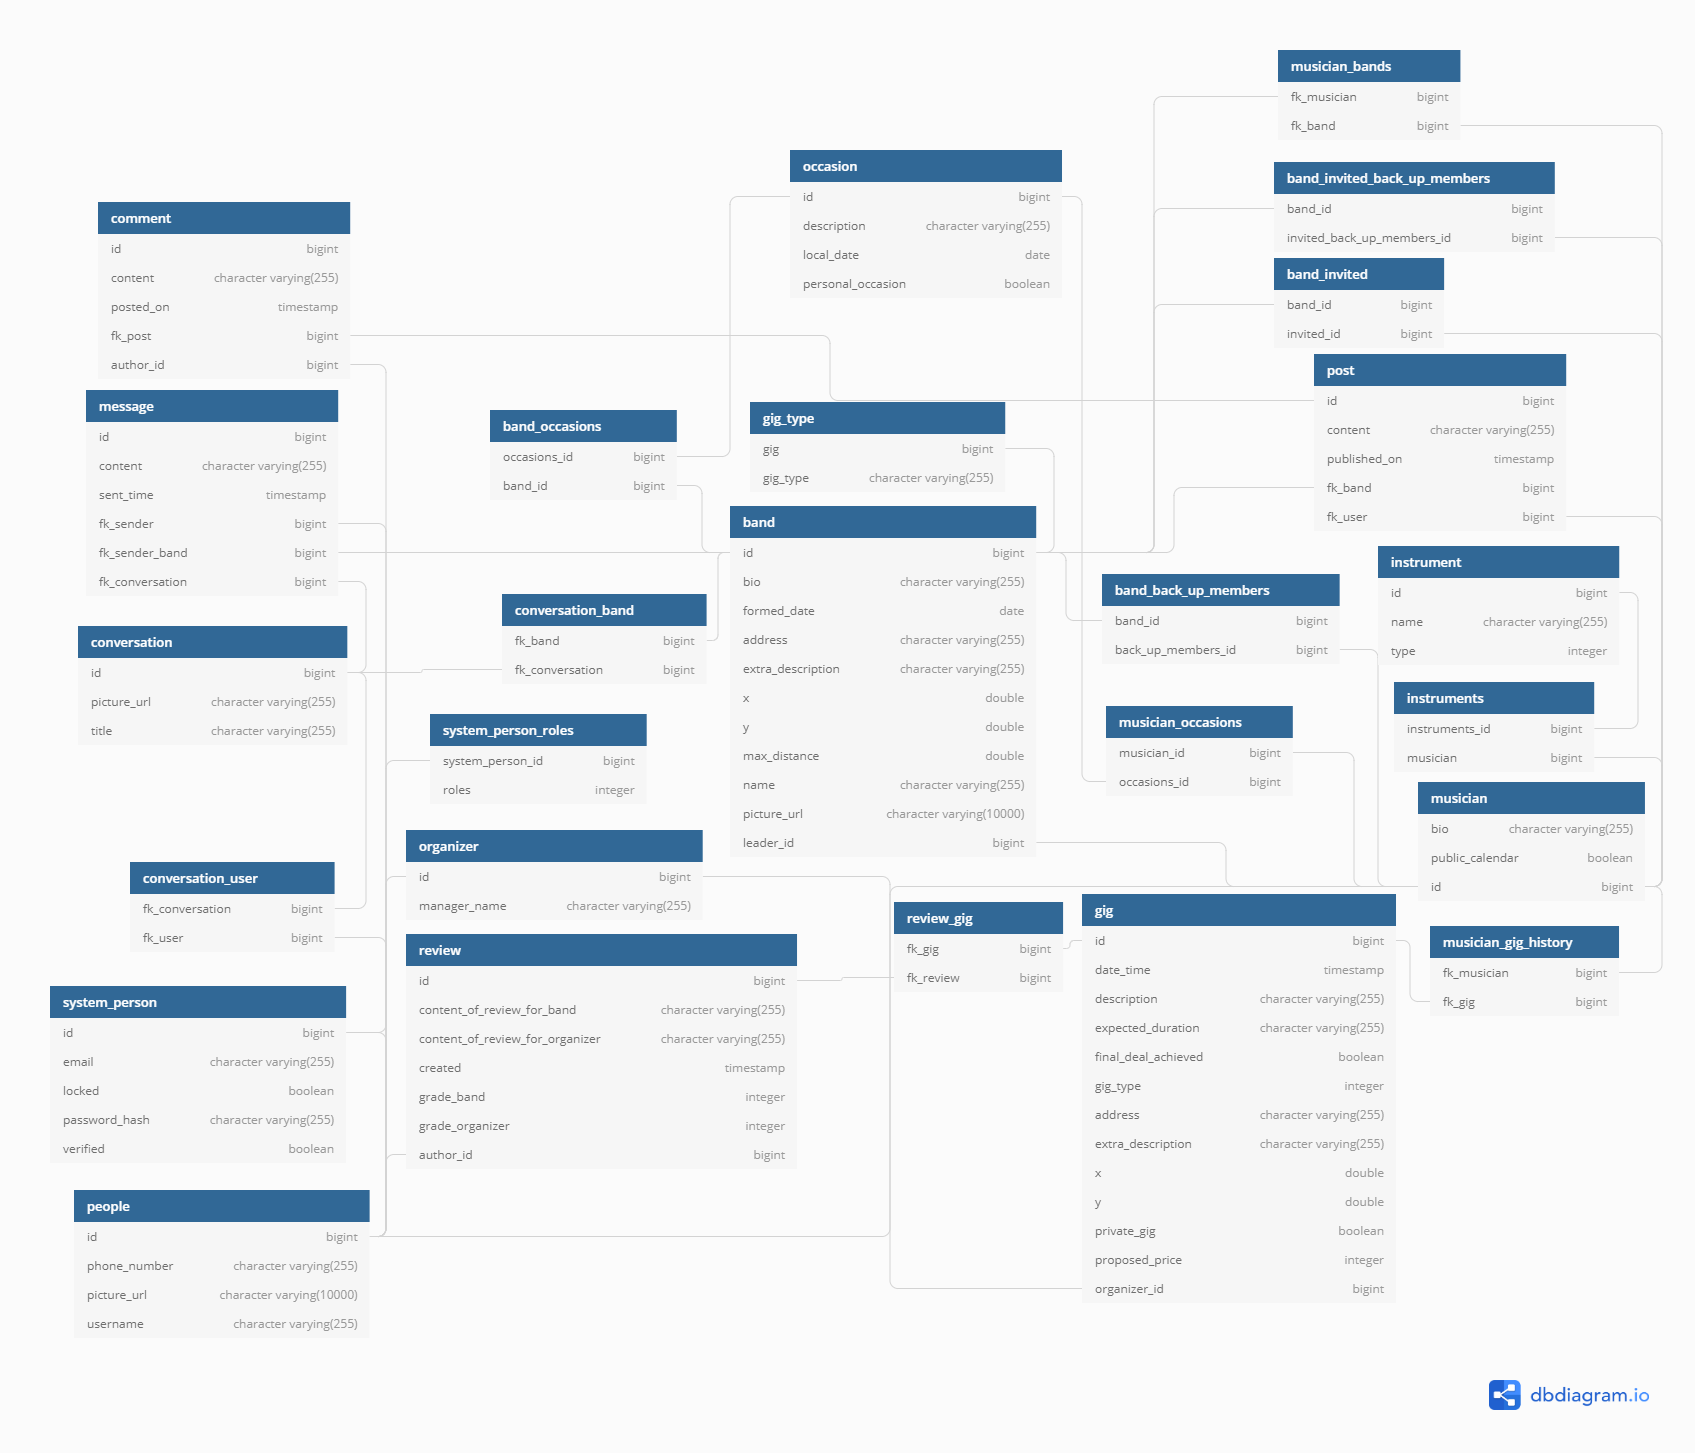
\includegraphics[width=17cm]{slike/ERModel.PNG}
			\end{center}
			\caption{Dijagram baze podataka}
			\label{fig:dijagramBaze}
		\end{figure}
			
			
			
		\section{Dijagram razreda}


			\textit{\textbf{dio 2. revizije}} \\
			
			\textit{Prilikom druge predaje projekta dijagram razreda i opisi moraju odgovarati stvarnom stanju implementacije} \\
			
			
			Na slici 4.3 prikazan je Controllers dio backend aplikacije. Controlleri su jedina izložena točka u aplikaciji te nad njima frontend izvršava upite. Svi Controller-i su zaštićeni Spring Security-jem te se prije svakog propuštanja zahtjeva na Controller autorizira token koji se nalazi u zaglavlju zahtjeva. Jedina iznimka su Controller-i koji služe za registraciju i prijavu. Nakon što se zahtjev autorizira Controller-i pozivaju servisni sloj aplikacije te od njih zahtjevaju da izvrše dio poslovne logike za koju su napisani. Povratni tip Controller-a su DTO-ovi (Data Transfer Objects) prikazani na slici 4.4. Njima se na frontend vraća samo dio informacije prikupljene od servisa.  

			\begin{figure}[H]
				\begin{center}
					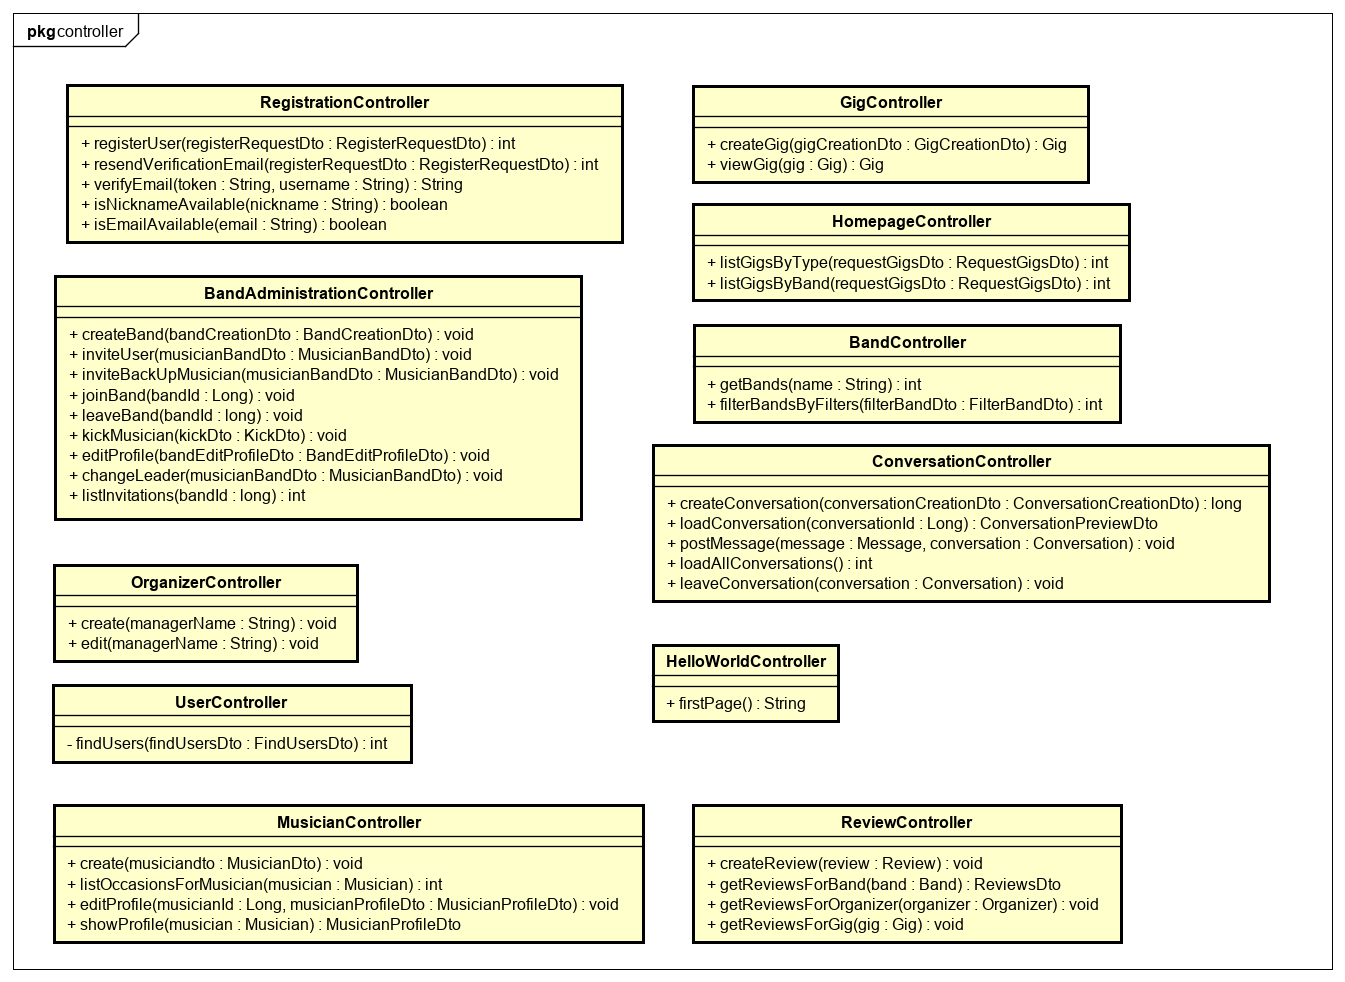
\includegraphics[width=17cm]{slike/kontroleri.PNG}
				\end{center}
				\caption{Dijagram razreda - dio Controllers}
				\label{fig:kontroleri}
			\end{figure}
		
			Slika 4.4 prikazuje DTO-ove kojima backend dio aplikacije komunicira s frontendom. DTO-ove smo modelirali tako da izbjegnemo kružne reference objekata koje dobijemo iz baze podataka. Kao posljedica, DTO-ovi sadrže uglavnom primitivne tipove ili neke druge DTO-ove (npr. ConversationPreviewDTO sadrži listu PersonPreviewDTO koji predstavljaju sudionike razgovora). DTO-ove koristimo u oba smjera komunikacije backenda i frontenda.
			
			
			\begin{figure}[H]
				\begin{center}
					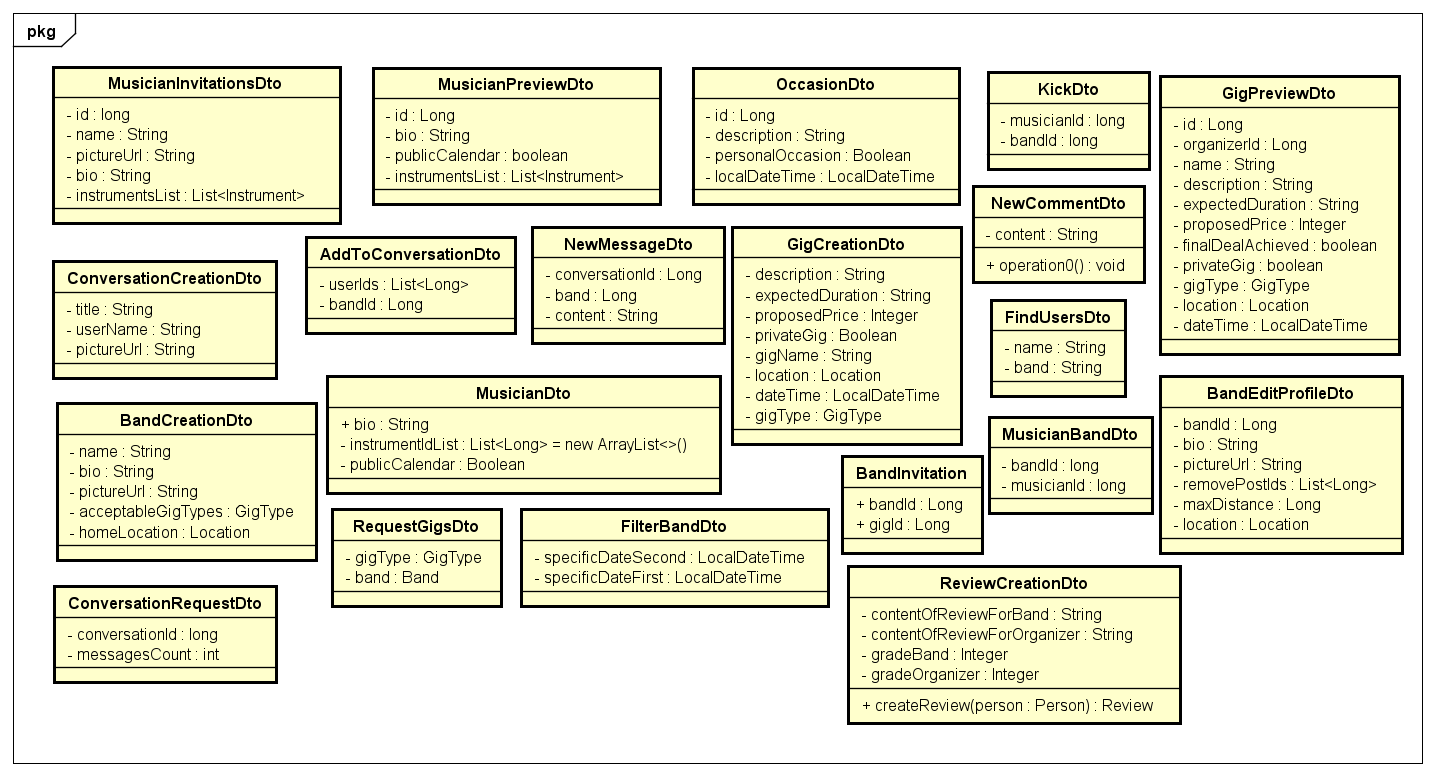
\includegraphics[width=17cm]{slike/nepovezani_dto.PNG}
				\end{center}
				\caption{Dijagram razreda - dio Data transfer objects, prvi dio}
				\label{fig:dto}
			\end{figure}
		
		Na ovom dijagramu prikazani su razredi Dto među kojima postoje veze jer pojedini razredi sadrže reference na druge razrede. 
		
		\begin{figure}[H]
			\begin{center}
				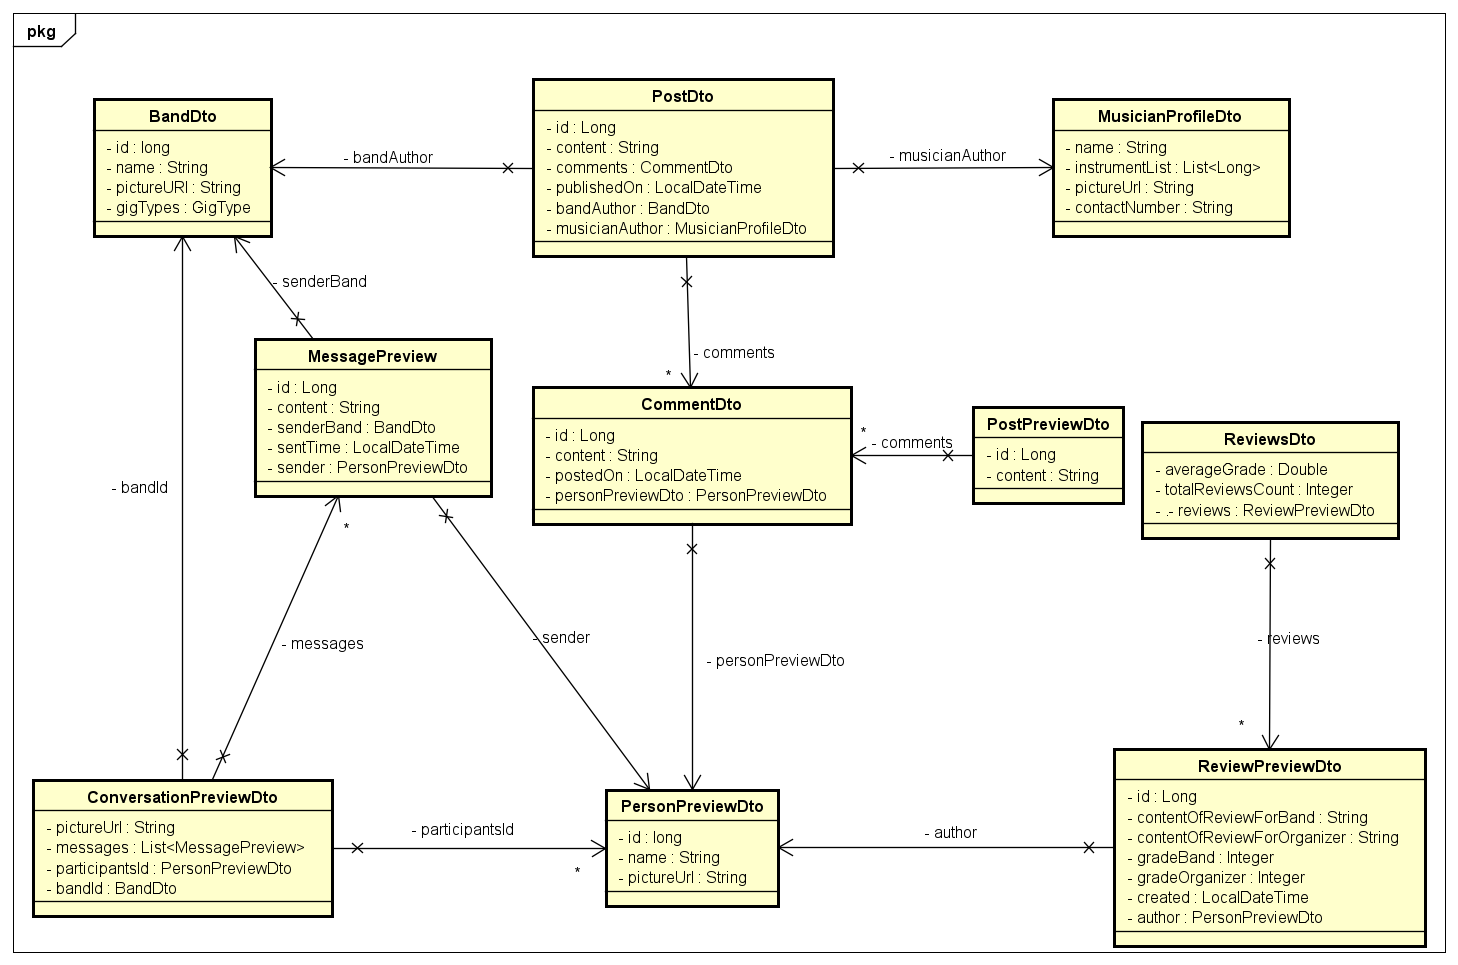
\includegraphics[width=17cm]{slike/povezani_dto.PNG}
			\end{center}
			\caption{Dijagram razreda - dio Data transfer objects, drugi dio}
			\label{fig:dto2}
		\end{figure}
		
		Slika 4.5 prikazuje dijagram razreda servisnog sloja. Servisi komuniciraju s repozitorijima koji pristupaju bazi i Controller-ima od kojih dobivaju i kojima vraćaju podatke. Servisi iz baze dobivaju instance objekata koji mogu biti povezani s drugim podatcima, itd. i njihov je cilj poštivajući poslovnu logiku obraditi te podatke i kao rezultat svog izvođenja vraćaju DTO-ove. Servisi sadrže svu poslovnu logiku. Gotovo svaki Controller ima pripadajući servis, a svaki je servis logički objedinjen skup funkcija poslovne logike. Iznimke koje se bacaju u servisima omataju se GigerException-om koji nasljeđuje RuntimeException. Ako se pogreška propagira iz sustava, možemo provjeriti njezin tip te ako je zamotana u GigerException, znači da je to iznimka koju smo očekivali, u protivnom je došlo do neočekivane situacije u sustavu.
		
		\begin{figure}[H]
			\begin{center}
				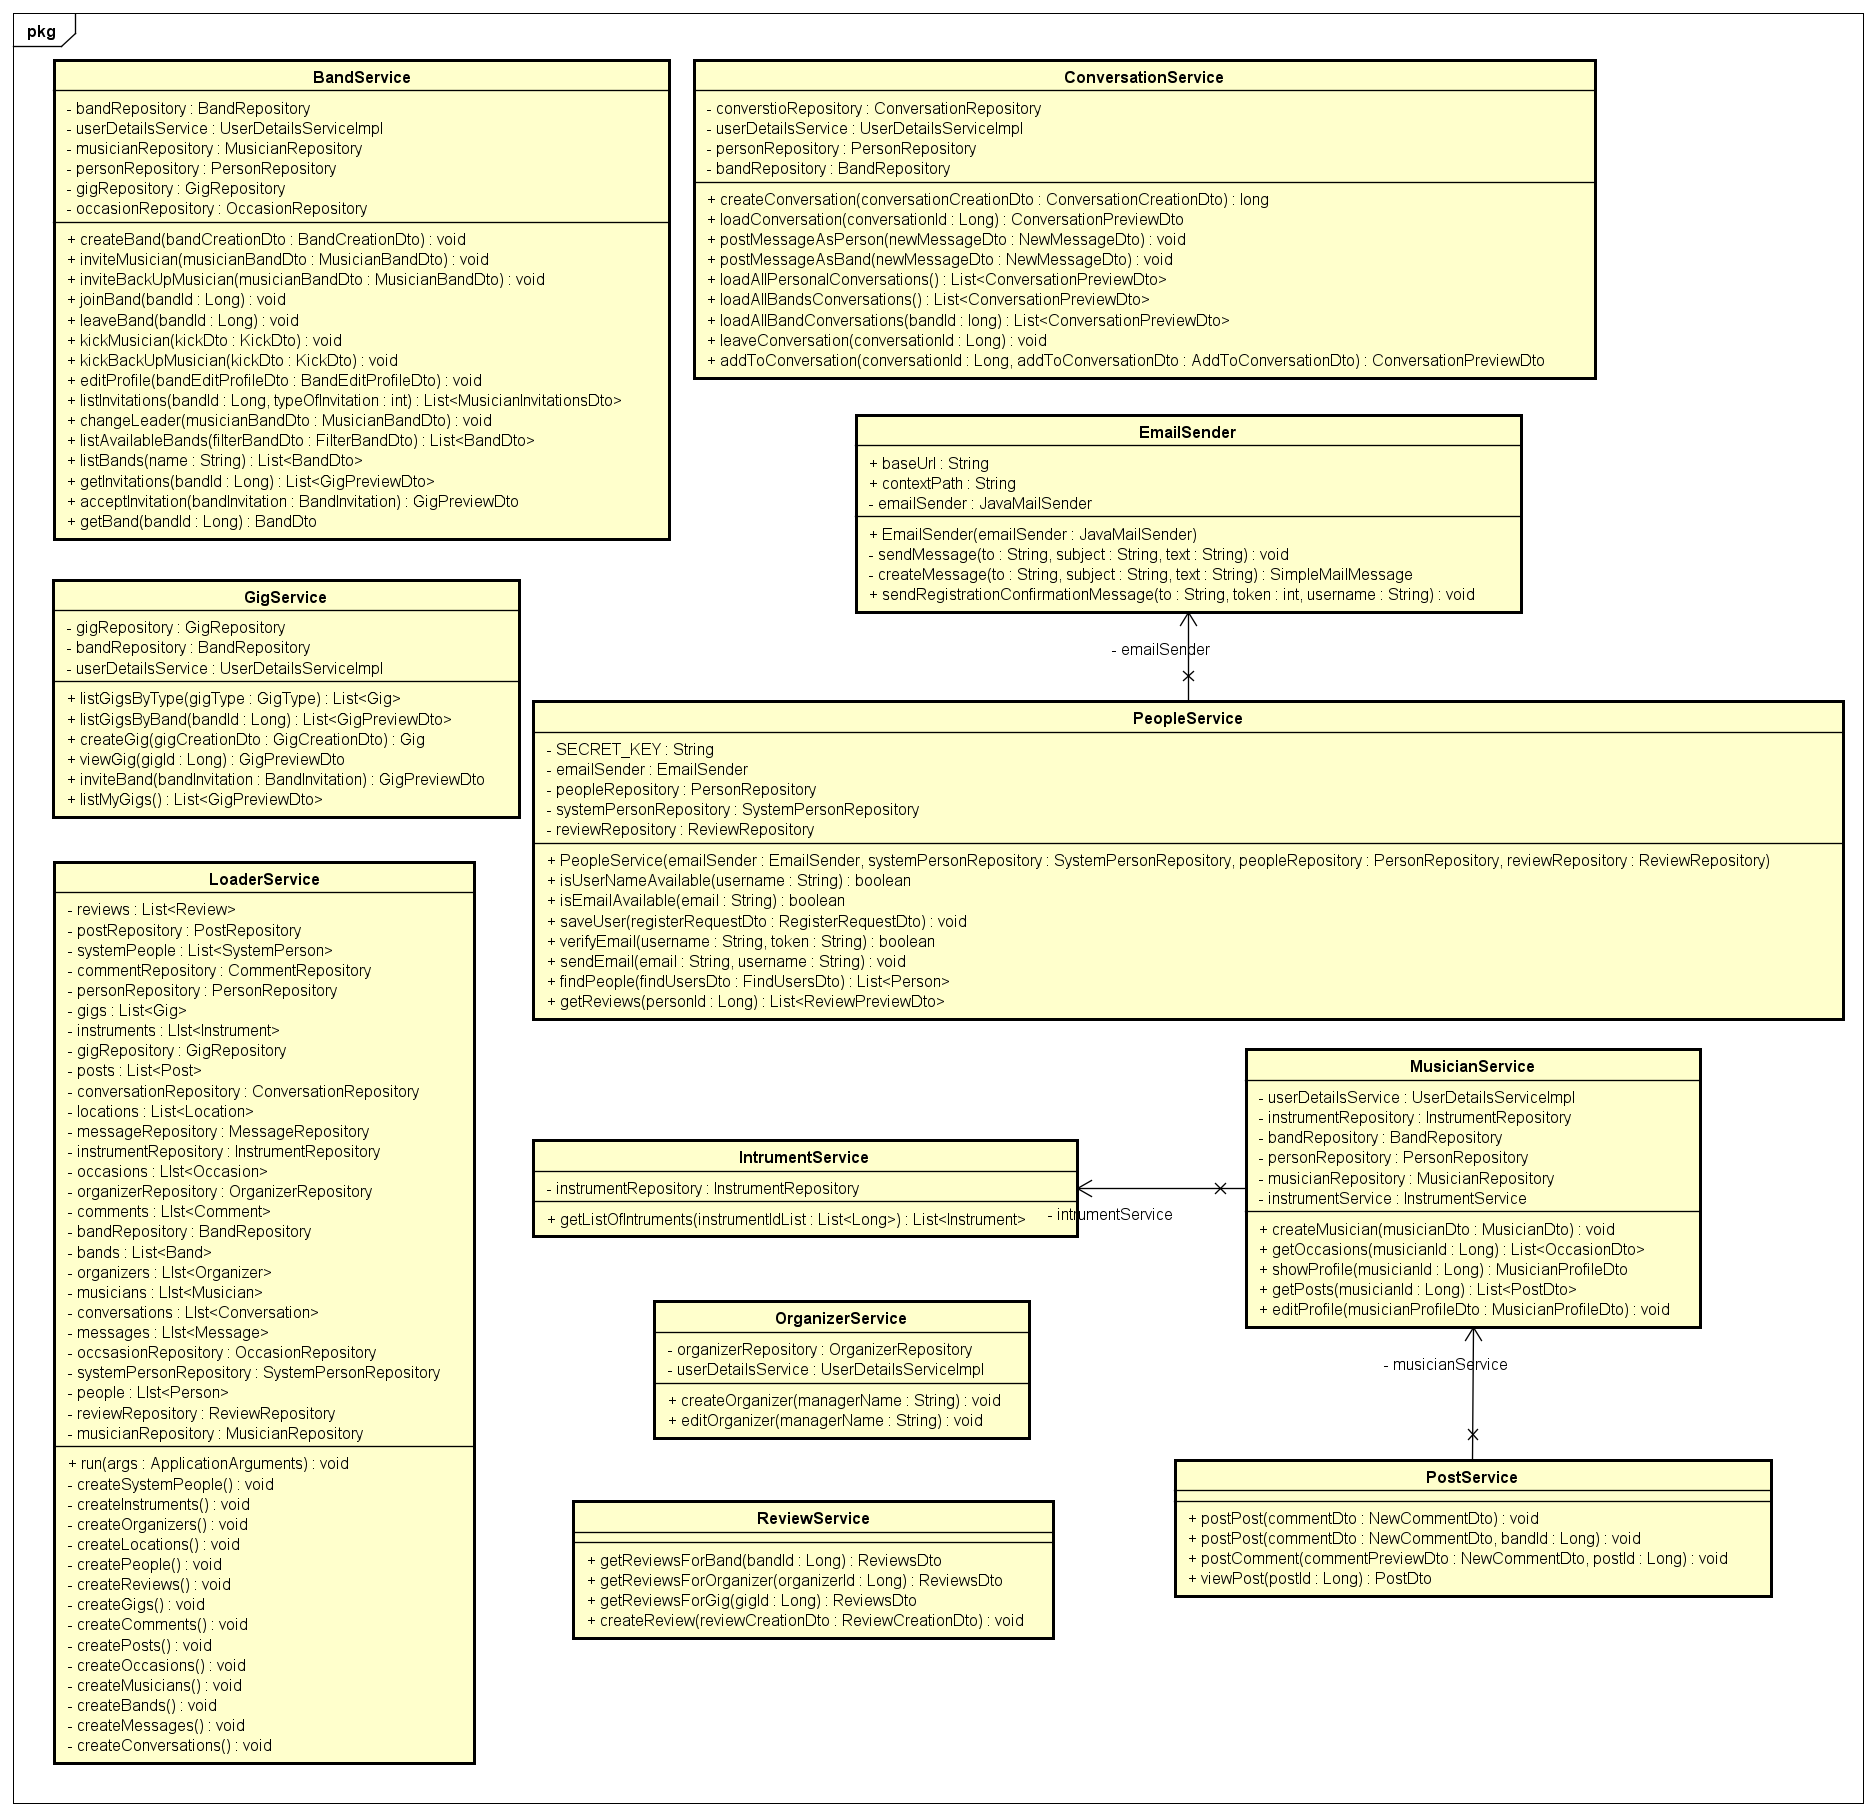
\includegraphics[width=16cm]{slike/service.PNG}
			\end{center}
			\caption{Dijagram razreda - dio Service}
			\label{fig:service}
		\end{figure}
	
	
	Slika 4.6 prikazuje razrede koji predstavljaju enitete enitetsko -  relacijskog modela u bazi podataka. Razred Band predstavlja bend kojim upravlja glazbenik koji je postavljen za voditelja benda. Razred SystemPerson predstavlja razred u kojem su objedinjeni svi sustavski podaci vezani za osobu kao što su: email, hash lozinke i id. Gig predstavlja  nastup nekog benda koji organizira određeni organizator i pri tom enkapsulira sve logističke informacije o tom nastupu. Razred Conversation omogućuje komunikaciju između aktora glazbenika i organizatora.
	Glazbenik je opisan razredom Musician, dok je organizator opisan razredom Organizer. Razredi Post, Comment, Location, Instrument, Message služe za enkapsulaciju informacija kako bi dopunili razrede poput Band, Conversation i Musician. GigType i Role predstavljaju enumeracije.
	
	
		\begin{figure}[H]
			\begin{center}
				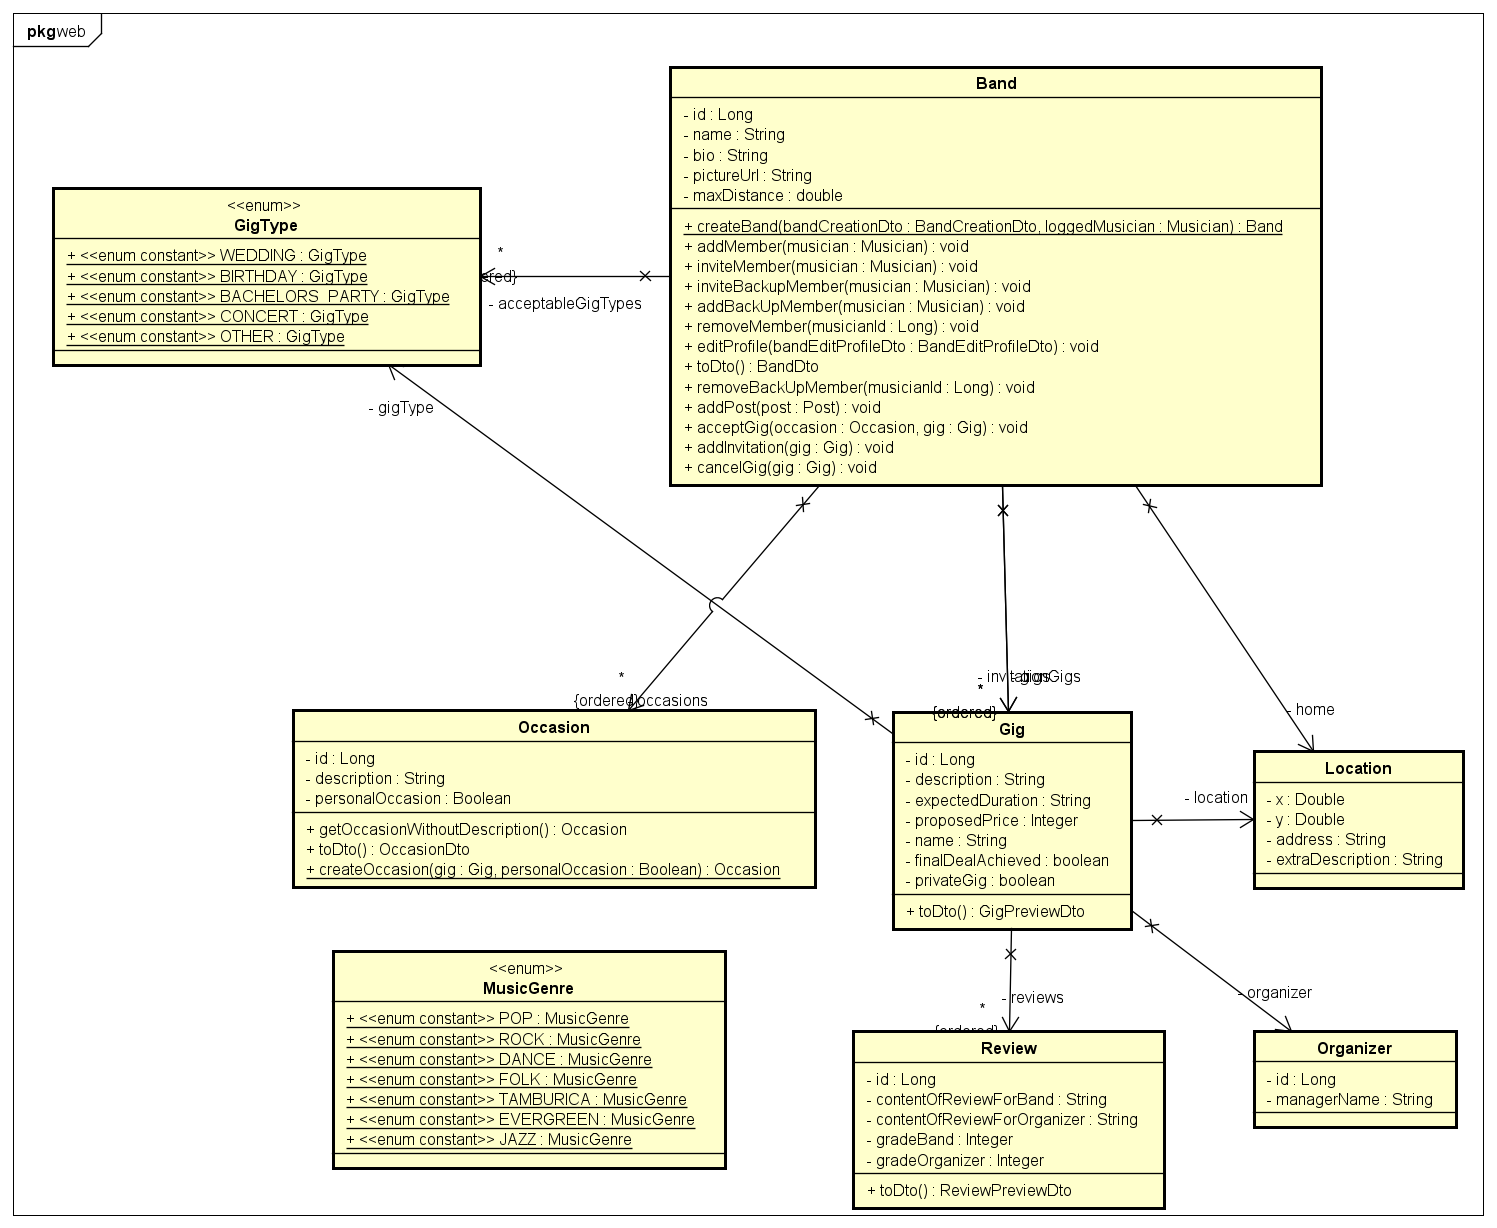
\includegraphics[width=17cm]{slike/entiteti_1.PNG}
			\end{center}
			\caption{Dijagram razreda - razredi entiteta 1}
			\label{fig:domena}
		\end{figure}
	
		\begin{figure}[H]
		\begin{center}
			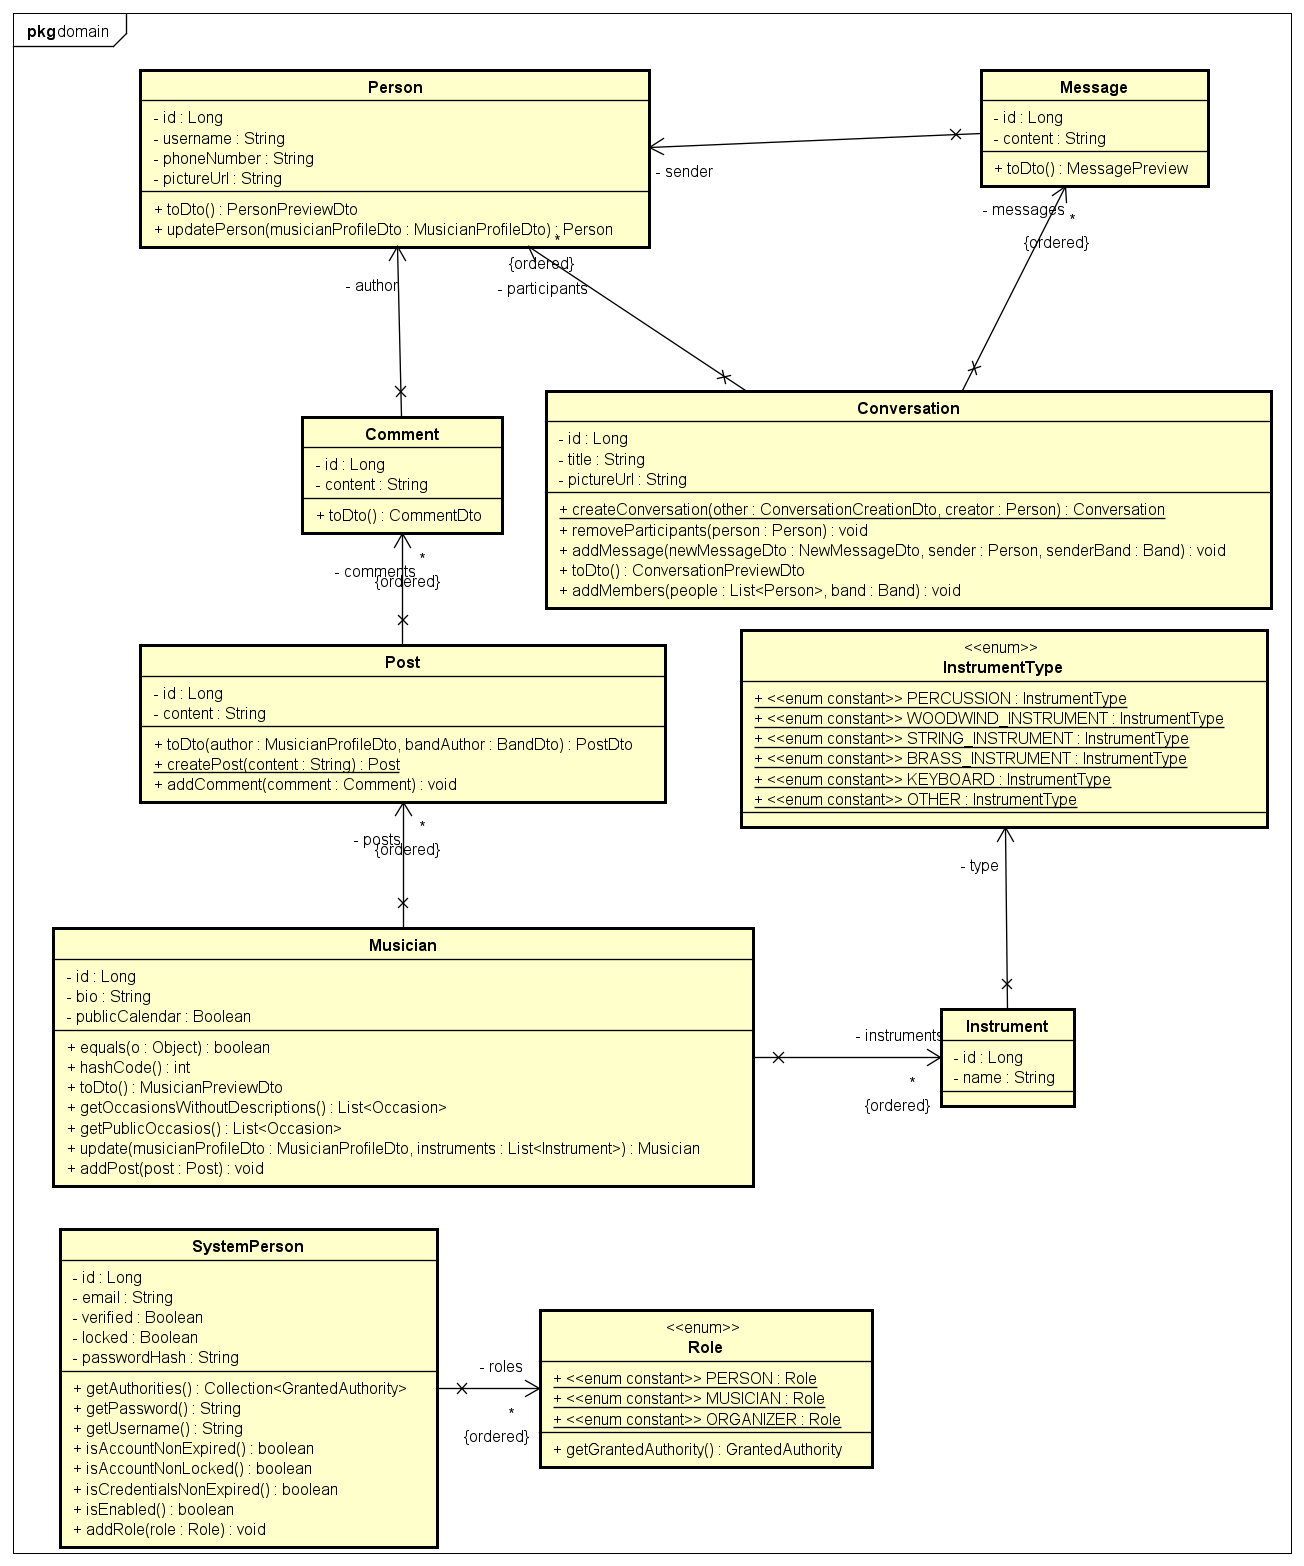
\includegraphics[width=17cm]{slike/entiteti_2.PNG}
		\end{center}
		\caption{Dijagram razreda - razredi entiteta 2}
		\label{fig:domena2}
	\end{figure}
	
	Na slici 4.7 prikazan je dijagram razreda zaduženih za Spring Security.
	Ulazna točka za autorizaciju zahtjeva je definirana u JwtRequestFilteru koji poziva UserDetailsServiceImpl da provjeri postoji li u bazi podataka zapis s akreditacijama koje se dekodiraju iz jwt tokena.
	AuthenticateController je zadužen za pružanje jwt tokena ukoliko u bazi pronađe zapis s odgovarajućim vrijednostima.
	Aplikacija ne pamti sesiju niti stanje (STATELESS) tako da korisnik prilikom postavljanja zahtjeva mora dostaviti svoj jwt token putem kojeg se autentificira i autorizira.
	JwtUtil klasa je puna pomoćnih metoda za baratanje jwt tokenom, a UserDetailsServiceImpl je posrednik između baze korisnika i AuthenticateControllera.
	Vezano uz autorizaciju, modelirana su tri DTO objekta koji definiraju objekte koje backend prima i daje kao zahtjev ili odgovor.
	

		\begin{figure}[H]
			\begin{center}
				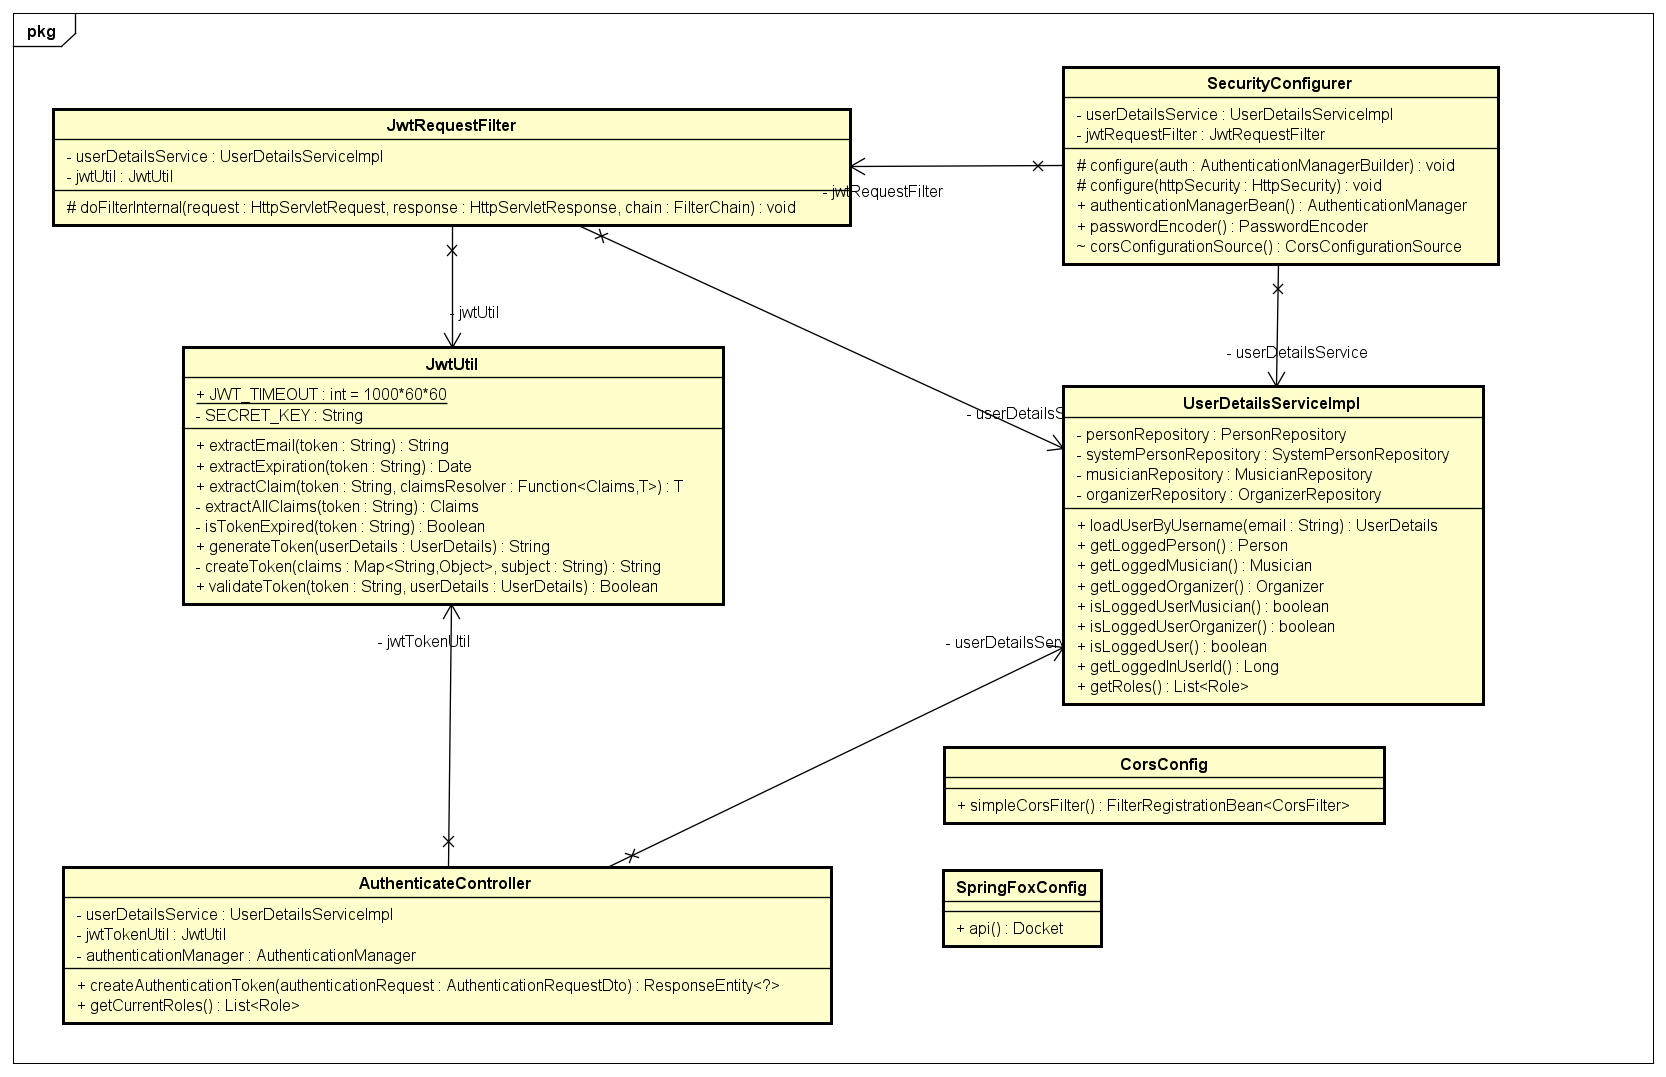
\includegraphics[width=17cm]{slike/security1.PNG}
			\end{center}
			\caption{Dijagram razreda - security}
			\label{fig:sec}
		\end{figure}
	
	Za dohvat podataka iz baze podataka koristimo Jakarta Persistence. Jakarta persistence je specifikacija programskog sučelja Java aplikacije koja opisuje upravljanje relacijskim podacima u aplikaciji. U ovoj aplikaciji za svaki entitet definiran je zasebni repozitorij koji nasljeđuje JpaRepositoryj. Jpa Repository sadrži osnovne metode za dohvat podataka, a Spring Boot omogućuje programeru da specificiranjem samo imena metode dobije implementaciju iste na korištenje. 
	
		\begin{figure}[H]
			\begin{center}
				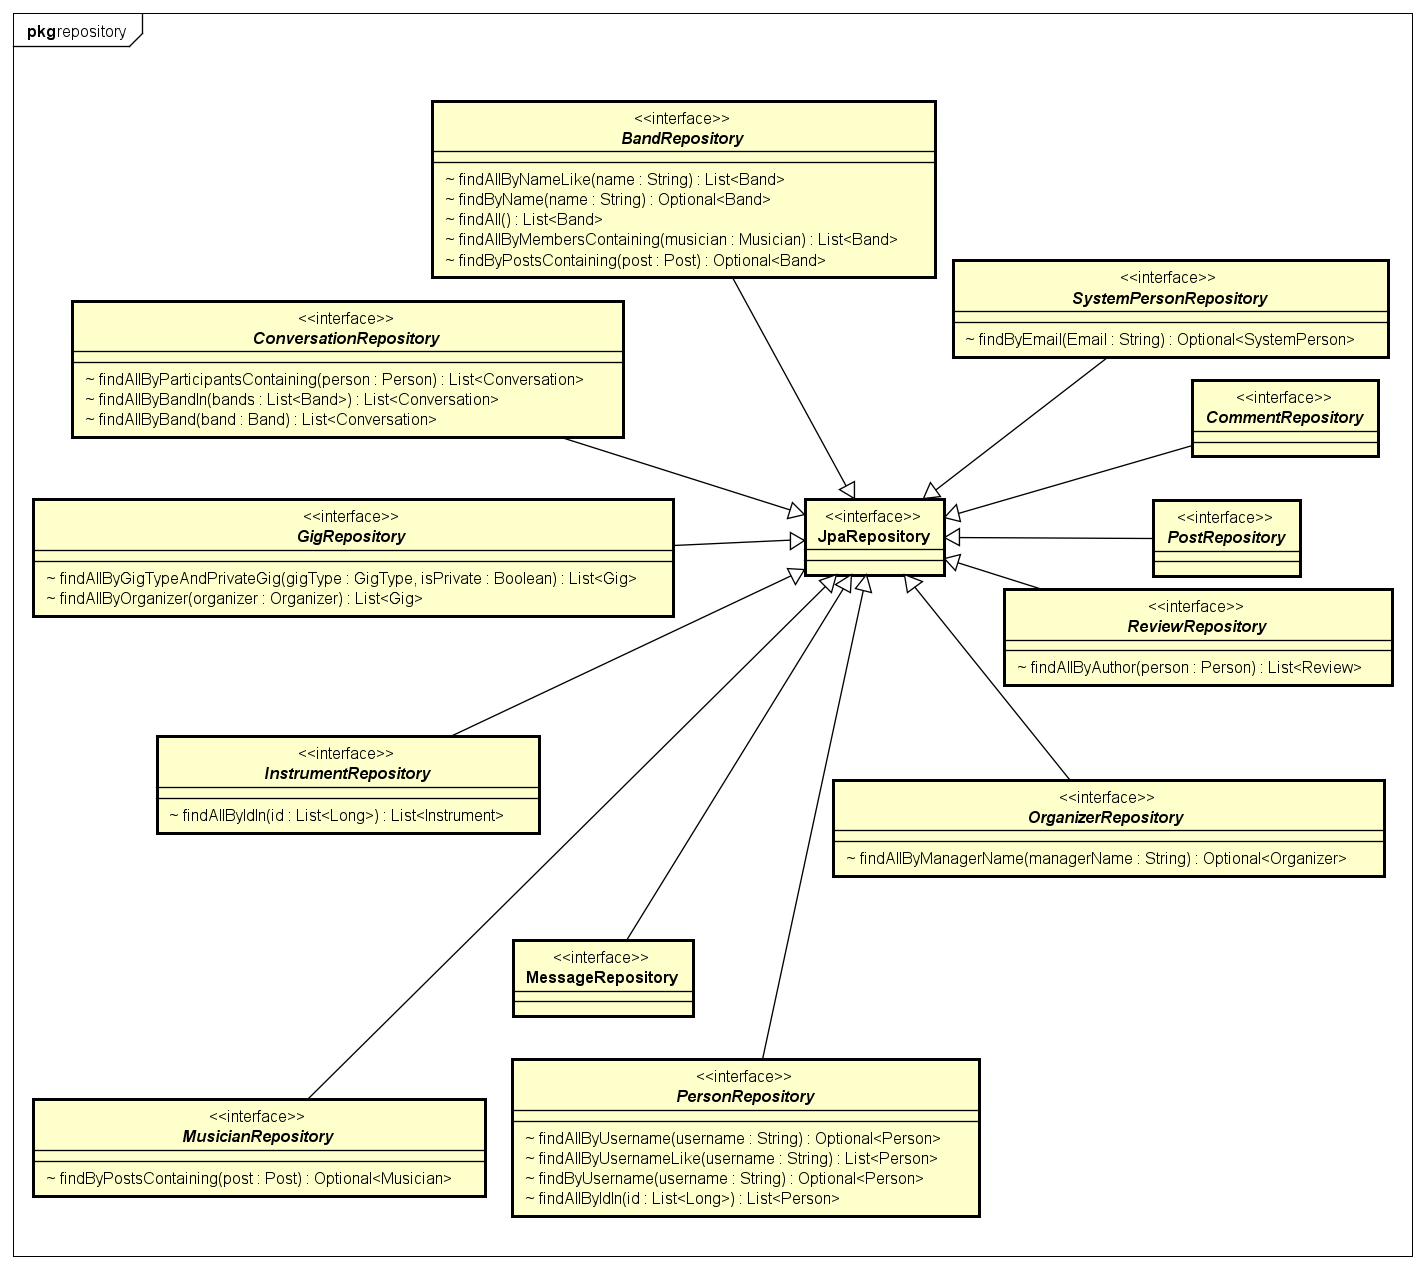
\includegraphics[width=17cm]{slike/repository1.PNG}
			\end{center}
			\caption{Dijagram repozitorija - repository}
			\label{fig:repository}
		\end{figure}
	
	Ovim dijagramom prikazane su moguće pogreške kao i iznimke. Pogreške se u ovom slučaju nalaze u Enumu Errorcode i služe za zaustavljanje operacija čijim izvođenjem se krši pravo pristupa ili se pokušava izvesti nemoguća akcija. Sve ostale logičke iznimke omotavaju se u iznimu GigerException. Za reprezentacijsko stanje prijenosa uvedena je iznimka RestExceptionHandler.
		
		\begin{figure}[H]
			\begin{center}
				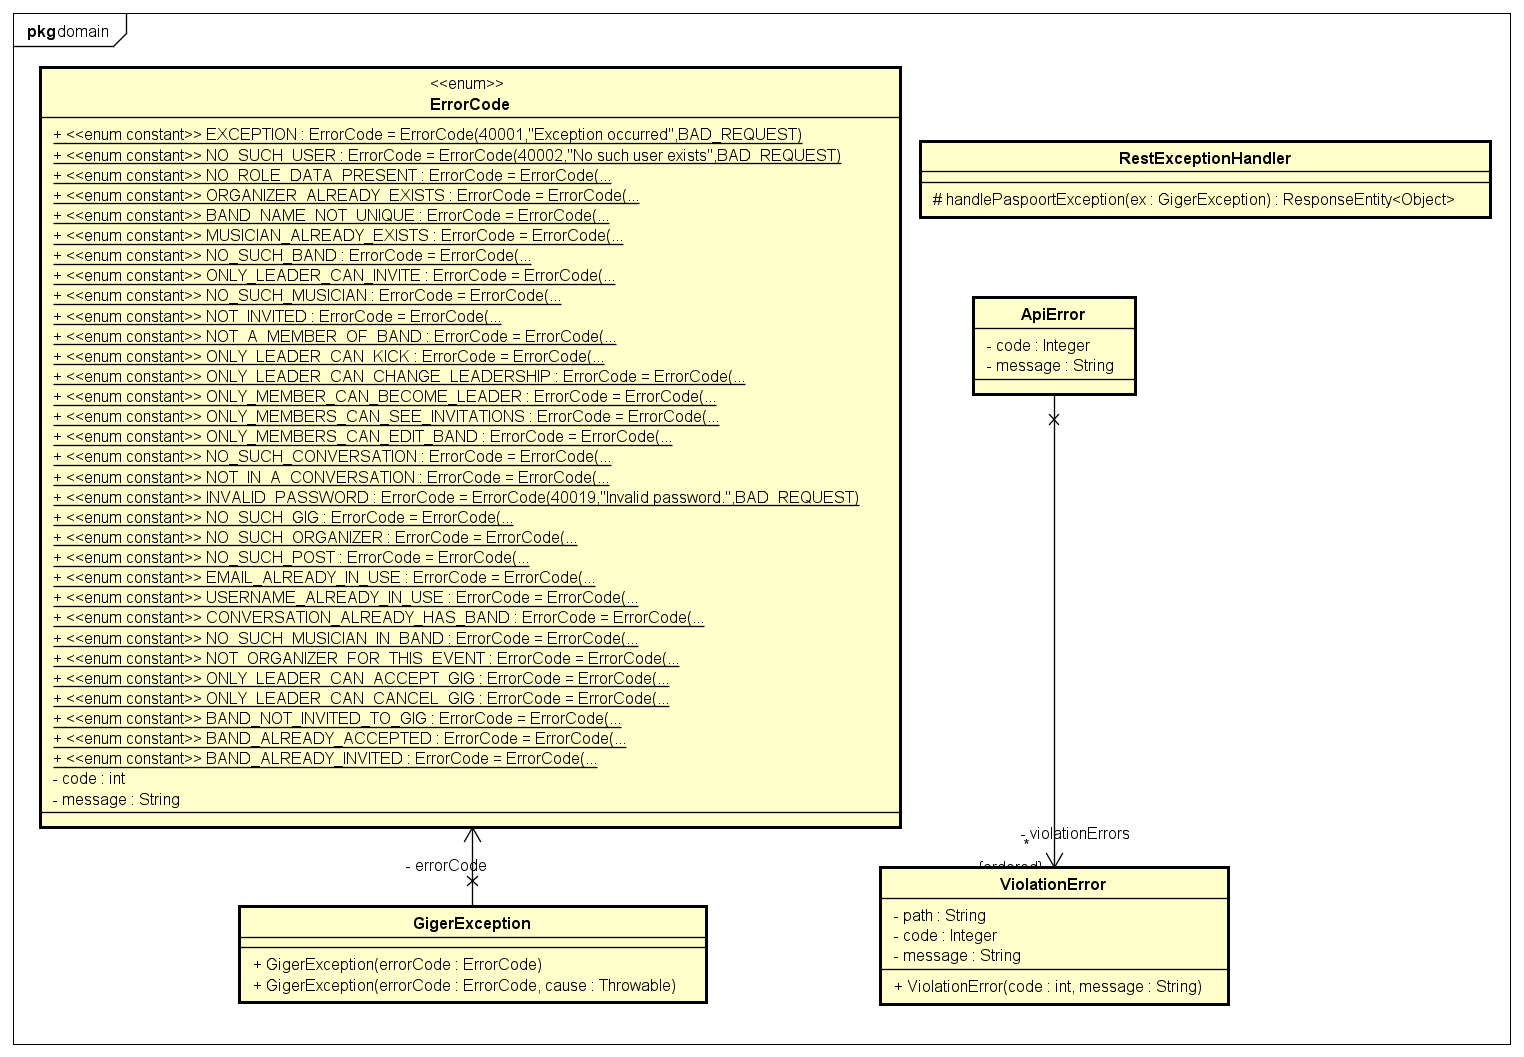
\includegraphics[width=17cm]{slike/errors1.PNG}
			\end{center}
			\caption{Dijagram razreda - errors}
			\label{fig:err}
		\end{figure}
	
		
	
	
	\eject
	
	\section{Dijagram stanja}
	
    Sljedeći dijagram stanja prikazuje stvaranje giga.Nakon uspješnog stvaranja giga, isti i dalje nije viđen pod opcijom "View public gigs". Da bi ostali korisnici mogli vidjeti taj gig, on prvo mora biti finaliziran.To znači da  organizator mora pozvati bend u svoj gig te nakon  što bend prihvati nastup ,gig postaje finaliziran (javan).
	
	
	
	
		\begin{figure}[H]
			\begin{center}
				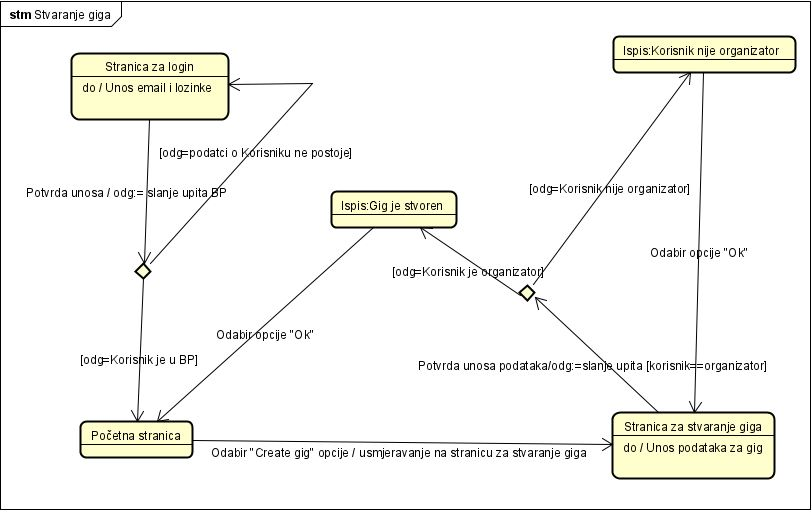
\includegraphics[width=17cm]{slike/stmStvaranjeGiga.JPG}
			\end{center}
			\caption{Dijagram stanja - stvaranje giga}
			\label{fig:stm}
		\end{figure}
	
	\eject
	
	
	\section{Dijagram aktivnosti}
	
	UML dijagram aktivnosti prikazuje detaljan tijek obrazaca uporabe, njegovu proceduralnu logiku te sudionike pojedinoga obrasca uporabe. 
	
	Na slici 4.11 prikazan je dijagram aktivnosti pisanja poruke. Korisnik se prijavi u sustav nakon čega odabire "Poruke". Nakon toga se iz baze dohvaćaju već postojeće poruke korisnika te mu ih aplikacija prikaže. Korisnik tada može ili započeti novi razgovor, ili odabrati postojeći. Ukoliko želi stvoriti novi razgovor, odabire opciju "Nova poruka" te mu aplikacija prikazuje praznu poruku. Nakon toga, odabire korisnika kojemu želi napisati poruku sve dok se on ne pronađe uspješno u bazi podataka. Ukoliko korisnik želi razgovarati s korisnikom s kojim je već vodio razgovor, odabire razgovor s tim korisnikom. Aplikacija iz baze dohvaća prošle poruke s odabranim korisnikom. U oba opisana slučaja, korisnik piše željenu poruku, odabire "Pošalji" nakon čega se poruka sprema u bazu te aplikacija prikaže potvrdu o slanju. 
	
	\begin{figure}[H]
		\begin{center}
			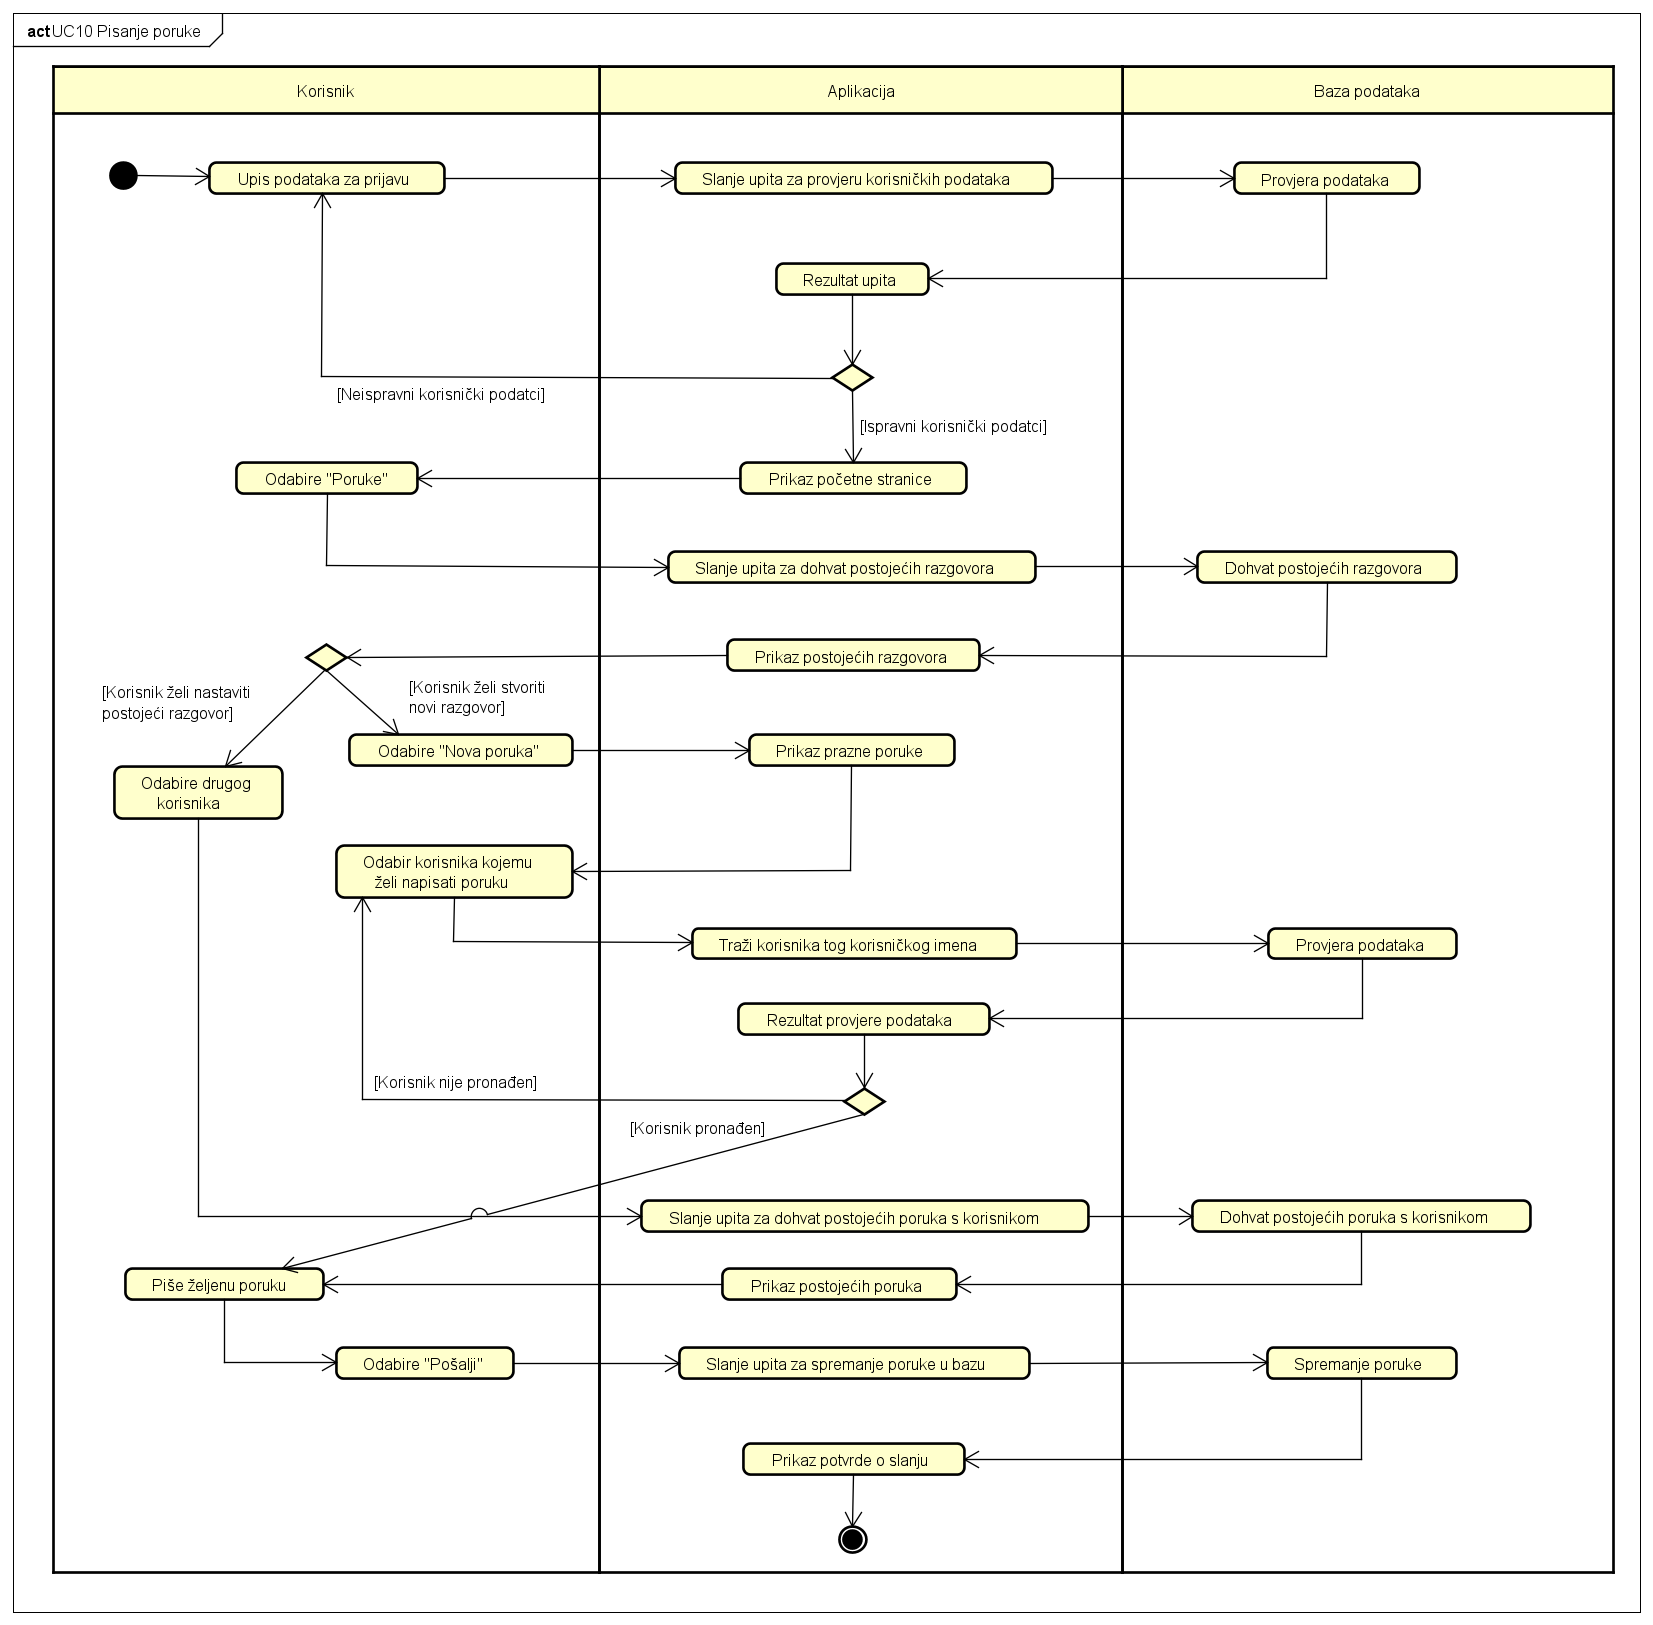
\includegraphics[width=17cm]{slike/dijagram_aktivnosti.PNG}
		\end{center}
		\caption{Dijagram aktivnosti}
		\label{fig:dijakt}
	\end{figure}
	
	\eject
	
	
	
	\section{Dijagram komponenti}
	
	Dijagram komponenti prikazuje zavisnost programskih komponenata i fizičku strukturu koda u terminima kodnih komponenti. Graf komponenti povezan je vezama ovisnosti kako bi se omogućila lakša analiza reakcije ostalih komponenti na promjene u jednoj komponenti. 
	Dohvat podataka iz SQL Postgres baze podataka vrši se sučeljima koja nasljeđuju JPA Repository pomoću SQL upita. Podaci koji pristižu iz baze podataka stavljaju se u DTO objekte koji se koriste u ostatku aplikacije. REST API šalje podatke iz backend aplikacije u obliku JSON-a frontend aplikaciji. Frontend aplikacija se sastoji od Javascript datoteka koje su grupirane u ovisnosti koji aktor im pristupa. Router je komponenta koja određuje koje datoteke se prikazuju klijentu. Sustavu se pristupa preko sučelja preko kojega mu se šalju HTML i JS datoteke iz frontend aplikacije.
	
	\begin{figure}[H]
		\begin{center}
			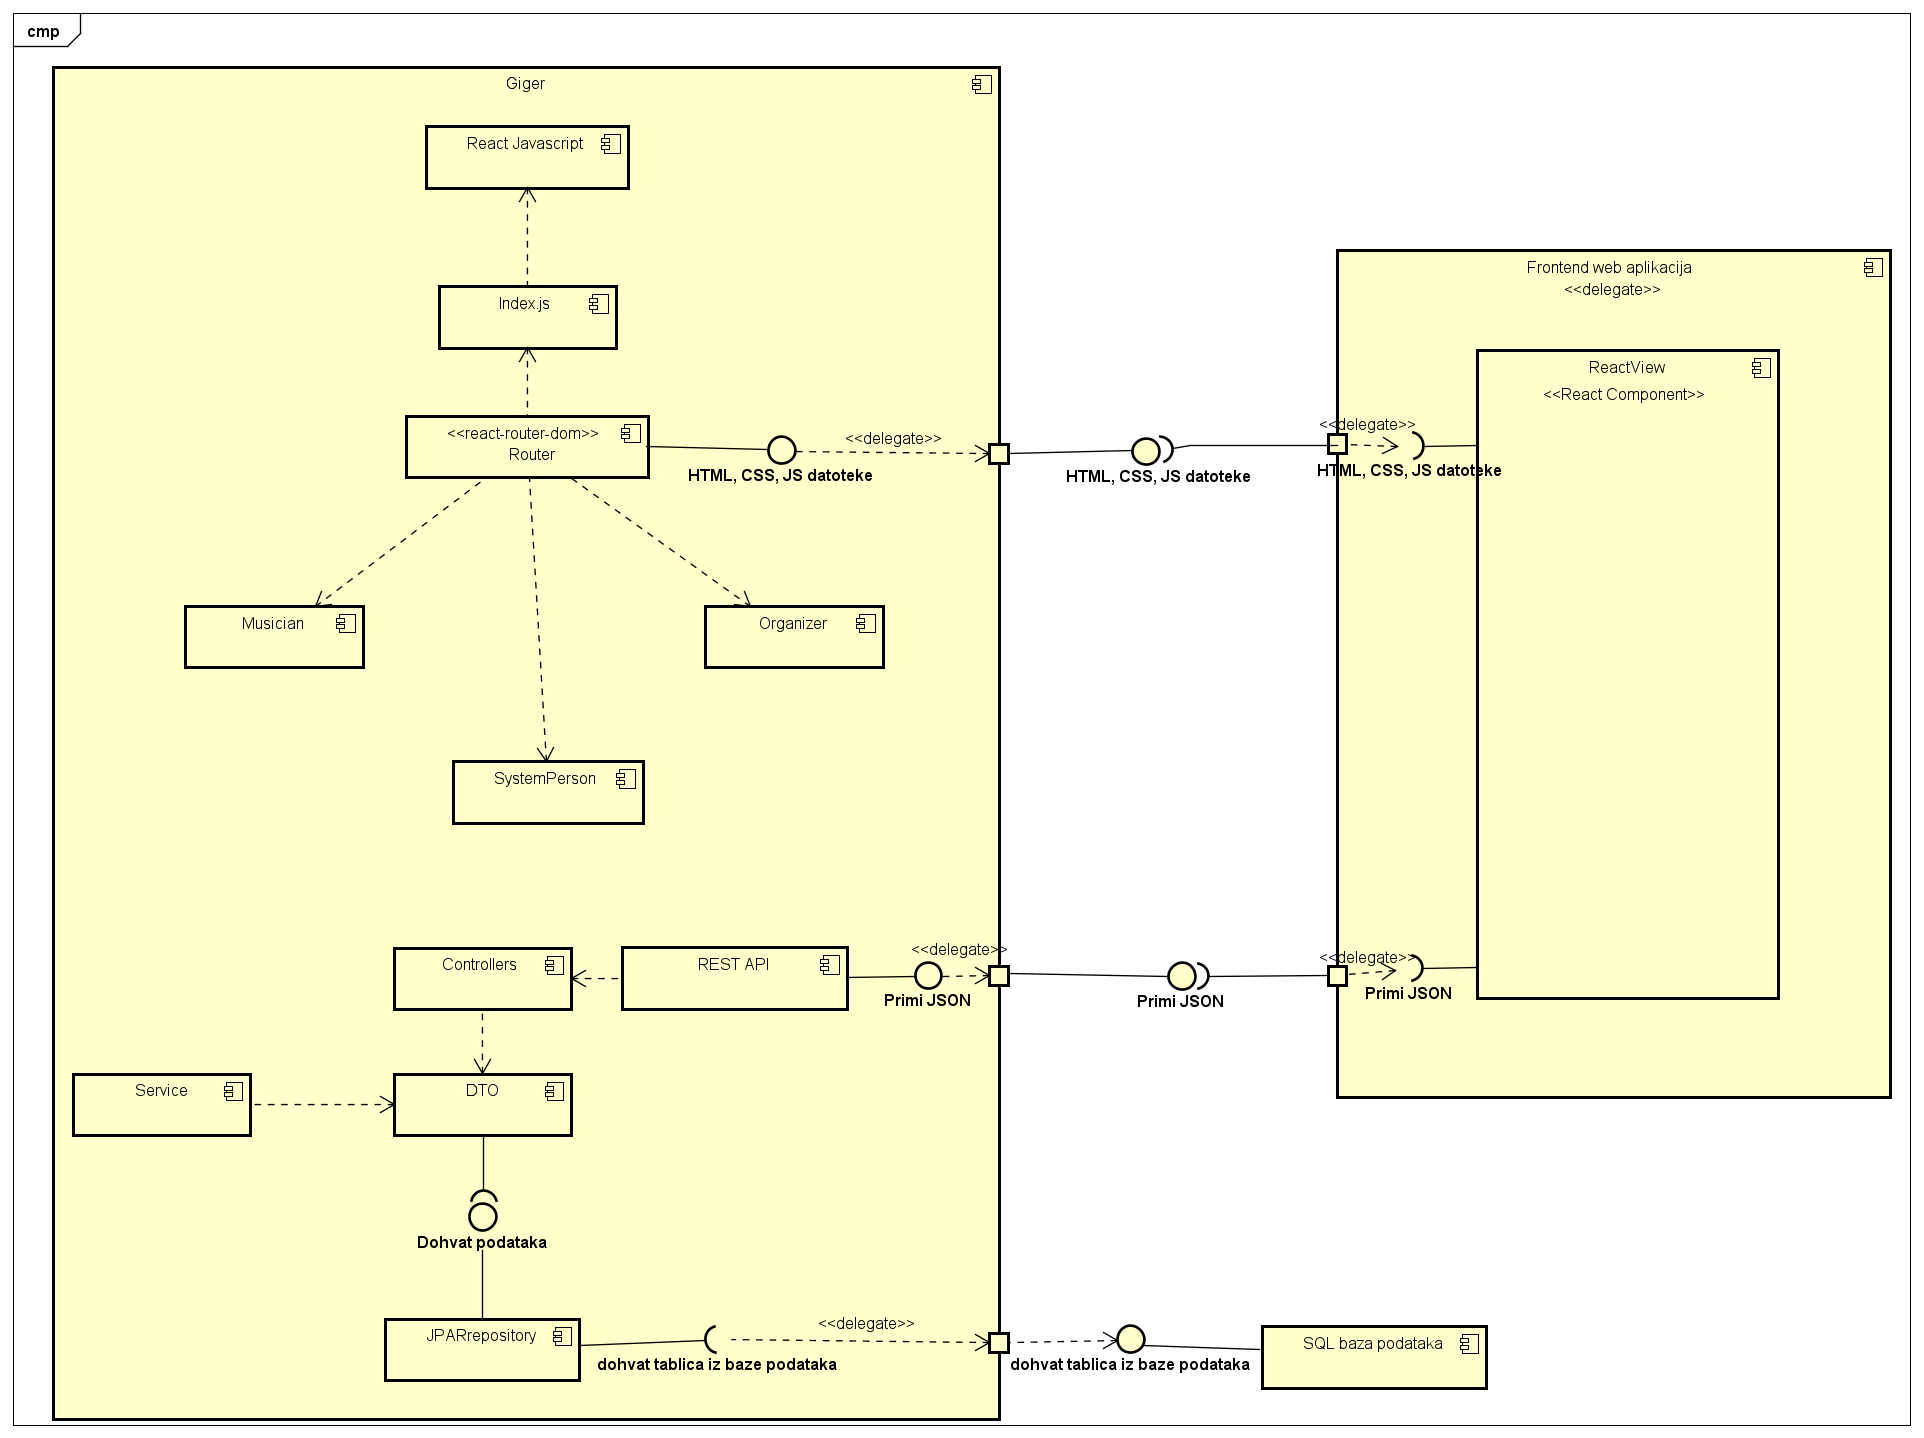
\includegraphics[width=17cm]{slike/compdig.PNG}
		\end{center}
		\caption{Dijagram komponenti}
		\label{fig:dijakt}
	\end{figure}
	
	\eject	
